\documentclass{article}

\usepackage[english]{babel}
\usepackage[margin=3cm]{geometry}
\usepackage{graphicx}
\usepackage{float}
\usepackage{caption}
\usepackage{hyperref}
\usepackage{amsmath}
\usepackage{wrapfig}
\usepackage[parfill]{parskip}

% fonts
\usepackage[T1]{fontenc}
\usepackage{helvet}
\renewcommand{\familydefault}{\sfdefault}

\graphicspath{{img/}}

\newtheorem{theorem}{Definition}[section]

\usepackage{enumitem}

\newenvironment{thmenum}
 {\begin{enumerate}[label=\upshape\bfseries(\roman*)]}
 {\end{enumerate}}

\usepackage{minted}
\setminted{frame=single,framesep=3pt,linenos}
\usepackage{upquote}
\usepackage{color}

\begin{document}

\begin{titlepage}
    \author{Tuur Vanhoutte}
    \title{Big Data}
\end{titlepage}

\pagenumbering{gobble}
\maketitle
\newpage
\tableofcontents
\newpage

\pagenumbering{arabic}

\section{Understanding Data Intensive Applications}

\subsection{Why Big Data?}

\subsubsection{Use case: data intensive application RouteYou}

\begin{figure}[H]
    \centering
    \includegraphics[width=0.5\textwidth]{routeyou.png}
    \caption{RouteYou}
\end{figure}

\begin{itemize}
    \item Routes - user preferences \& interests
    \item Searcheable Text data
    \item Geospatial data
    \item Community driven
    \begin{itemize}
        \item Exponential user growth is necessary to make the application posssible
        \item Server power/bills should grow linearly
    \end{itemize}
\end{itemize}

\subsection{Data Intensive Application: RAMS!}

\begin{itemize}
    \item \textbf{Reliable}
    \begin{itemize}
        \item tolerating human mistakes
    \end{itemize}
    \item \textbf{Available}
    \item \textbf{Maintainable}
    \begin{itemize}
        \item Easy to adapt (evolvability)
        \item Easy to deploy \& operate (operations/sys admins)
    \end{itemize}
    \item \textbf{Scalable}
    \begin{itemize}
        \item User growth while maintaining low response times
    \end{itemize}
\end{itemize}

\subsubsection{Common similar abbreviations}

\begin{itemize}
    \item Infrastructure: RAS (Reliable, Available, Serviceable)
    \item Developer: RMS (Reliable, Maintainable, Scalable)
\end{itemize}

\subsubsection{Methods to improve Maintainability}

\begin{itemize}
    \item Github
    \item Error handling
    \item Relative paths (not absolute)
    \item Abstraction (REST API, \dots)
    \item Documentation
\end{itemize}

\subsubsection{RAMS applied to RouteYou application}

\begin{itemize}
    \item Geospatial data (longitude, latitude)
    \item Available \& scalable
    \item Scalable \& low response time
    \item Community driven - unstructured text
    \item Maintainable: automatic classification of community input (ML)
\end{itemize}

\begin{figure}[H]
    \centering
    \includegraphics[width=0.5\textwidth]{RAMS-routeyou.png}
    \caption{To support many users, you need a caching layer}
\end{figure}


\subsection{Learning outcome for this module}

Being able to make infrastructure \& software choices to 
build a Reliable, Available, Maintainable \& Scalable (RAMS) 
data intensive application.

\begin{itemize}
    \item Deep insights into database technology \& cloud services
    \item Connecting with Machine Learning \& AI
    \item Configuring a data back-end (in the cloud or locally)
\end{itemize}


\subsection{Scaling}
\subsubsection{MySQL scaling}

\begin{figure}[H]
    \centering
    \includegraphics[width=0.5\textwidth]{mysql-scaling.png}
    \caption{Transactions/sec }
\end{figure}

\begin{itemize}
    \item Processing power of 16-64 = slightly less then 4x
    \item Real performance: 2.3x
    \item = scaling up: add more processing power to the system
\end{itemize}

\subsubsection{ElasticSearch Scaling: distributed system}

\begin{figure}[H]
    \centering
    \includegraphics[width=0.5\textwidth]{elasticsearch-scaling.png}
    \caption{Response time per request}
\end{figure}

\begin{itemize}
    \item Scaling out: add more servers to your data system
\end{itemize}

\subsubsection{Professional architecture (Dev oriented)}

\begin{figure}[H]
    \centering
    \includegraphics[width=0.5\textwidth]{professional-architecture.png}
    \caption{Professional architecture diagram}
\end{figure}


\begin{itemize}
    \item \textbf{Reverse proxy / Load balancer:} improves scalability
    \item \textbf{Opcode/app/Webserver:} webservice + API
    \item \textbf{Key-value store:} `caching layer'
    \item \textbf{Database server:} distributed storage system + relational database
\end{itemize}

\subsubsection{Time series Distributed database (OpenTSDB, InfluxDB)}

\begin{figure}[H]
    \centering
    \includegraphics[width=0.5\textwidth]{time-series-distributed-db.png}
    \caption{Data from windmill sensors. Most sensors log about every second}
\end{figure}

\begin{itemize}
    \item Losing data is not that big a problem
    \item Massive amount of data to write 
\end{itemize}

\subsection{Scalability \& application performance management}

Response times and percentiles rule the web

\subsubsection{The need for speed: some insights from Google}

\begin{itemize}
    \item Speed is a ranking factor
    \item When your site has high response times, less URLs will be crawled from your site
    \item 53\% of visits are abandoned if a site takes longer than 3 seconds to load
    \item Slow websites will be labeled by Google Chrome
\end{itemize}

\subsubsection{Response times for websites}

\begin{itemize}
    \item \textbf{Ideal:} `blink of an eye' is 300-400 ms
    \item \textbf{Excellent:} 500ms to 1.5 seconds at most
    \item \textbf{Barely acceptable:} 3 seconds
\end{itemize}

Response time = Network latency + processing

\begin{itemize}
    \item 2.9 seconds is faster than 50\% of the web
    \item 1.7 seconds is faster than 75\% of the web
    \item 0.8 seconds is faster than 94\% of the web
\end{itemize}

\subsubsection{4 components of network latency}

\begin{figure}[H]
    \centering
    \includegraphics[width=0.7\textwidth]{network-latency.png}
    \caption{Network latency diagram}
\end{figure}

\begin{itemize}
    \item \textbf{Processing delay}
    \begin{itemize}
        \item Processing network software stack (TCP/IP layers)
        \item Routing decisions
    \end{itemize}
    \item \textbf{Transmission delay}
    \begin{itemize}
        \item Bits on physical link (Bandwidth plays a big role, ex: 1Gbit/s)
    \end{itemize}
    \item \textbf{Propagation delay}
    \begin{itemize}
        \item Speed of EM signals in fiber: 200.000 km/s (67\% of lightspeed)
        \item Changes with distance and medium (Copper: 64\% of lightspeed)
    \end{itemize}
    \item \textbf{Queing delay}
    \begin{itemize}
        \item Time spent in router \& NIC buffers
    \end{itemize}
\end{itemize}

\subsubsection{TCP Congestion Window - slow start}

\begin{itemize}
    \item Network congestion = a network node or link is carrying more data than it can handle
    \item The internet is built around dropped packages
\end{itemize}

\begin{figure}[H]
    \centering
    \includegraphics[width=0.5\textwidth]{tcp-congestion-window.png}
    \caption{TCP Congestion window}
\end{figure}

\begin{itemize}
    \item 4-8-16-32 TCP segments (Win 2008, Win7)
    \item 10-20-40 (Linux 2.6+, Windows Server 2016 / Windows 10)
\end{itemize}

\begin{figure}[H]
    \centering
    \includegraphics[width=0.5\textwidth]{tcp-handshakes.png}
    \caption{Because of many handshakes, there is a lot of latency}
\end{figure}

\begin{itemize}
    \item Solution: KeepAlive of a HTTP Persistent Connection
    \begin{itemize}
        \item Only one 3-way handshake for many requests
        \item Lower network \& CPU load
        \item Lower response times
        \item \textbf{Downside}: more connections open $\Rightarrow$ more memory, more connection failures, app crashing, \dots
    \end{itemize}
\end{itemize}

\begin{itemize}
    \item Measure parallel requests of a website using \url{https://www.webpagetest.org/}
    \item Get a waterfall view of a webpage
\end{itemize}

\subsubsection{Long tail latency}

\begin{figure}[H]
    \centering
    \includegraphics[width=0.5\textwidth]{long-tail-latency.png}
    \caption{Long tail latency vs Normal latency}
\end{figure}


\begin{itemize}
    \item The average latency doesn't show the whole picture
    \item Long tail latency = 99th percentile highest latency
    \begin{itemize}
        \item To be experienced by a lot more than 1\% of users!
    \end{itemize}
    \item Best customers encounter highest percentiles
    \item URL consists of many requests
\end{itemize}

\subsection{Conclusion}

\begin{itemize}
    \item Our goal is RAMS (or RASS)
    \item Many data models \& stores: transactional, timeseries, text search
    \item Website 99th percentile + DNS + TCP $\Rightarrow$ < 2s response time
    \begin{itemize}
        \item Efficient caching
        \item Think about your architecture (infrastructure + software) before coding
    \end{itemize}
\end{itemize}

\section{Professional storage}

\subsection{Cloud MIPS}

\begin{figure}[H]
    \centering
    \includegraphics[width=0.75\textwidth]{mips.png}
    \caption{MIPS = Million Instructions Per Second}
\end{figure}

\subsection{Latency vs storage space pyramid}

\begin{figure}[H]
    \centering
    \includegraphics[width=0.75\textwidth]{latency-vs-storage-space-pyramid.png}
    \caption{The higher the performance, the higher the cost per byte of storage}
\end{figure}

\subsection{Storage media}

\subsubsection{Magnetic disks}

\begin{figure}[H]
    \centering
    \includegraphics[width=0.5\textwidth]{magnetic-disks.png}
    \includegraphics[width=0.4\textwidth]{magnetic-disks-performance.png}
    \caption{Massive capacity but mechanical latency}
\end{figure}

\begin{itemize}
    \item Seek time and latency are the key bottlenecks
    \item Need large quantity of disks for good server performance
\end{itemize}

\subsubsection{Flash (NAND) / SSDs}

\begin{figure}[H]
    \centering
    \includegraphics[width=0.5\textwidth]{flash-nand.png}
    \caption{Flash storage}
\end{figure}

\begin{itemize}
    \item SSD = Solid State Drive
    \item NAND = MOSFET + floating gate
    \item Voltage between control gate and N+ : electrons in floating gate
    \item This works very quickly
\end{itemize}

\textbf{Architecture}

\begin{itemize}
    \item Page = 4 KB, pages are in block
    \item Block = 128 pages (4KB * 128 = 512 KB)
    \item You can read or write page per page
    \item Erasing has to erase the entire block
\end{itemize}

\begin{figure}[H]
    \centering
    \includegraphics[width=0.5\textwidth]{flash-architecture.png}
    \caption{Diagram of a flash Block}
\end{figure}


\subsubsection{Big difference between read and writing}

\begin{figure}[H]
    \centering
    \includegraphics[width=0.5\textwidth]{nand-read-write.png}
    \caption{Reading \& writing on Flash storage}
\end{figure}

\begin{itemize}
    \item Limited number of writes
    \item Slow block write
    \item Limited `normal' write (programming)
\end{itemize}

\subsubsection{IOPS vs Bandwidth}

\begin{itemize}
    \item Transactions \& virtualized workloads: lots of random access
    \item Timeseries fileserving: mostly sequential
    \item HDD: random performance can be extremely low to medium 
    \item IOPS = Input/Output Operations Per Second
\end{itemize}

\begin{figure}[H]
    \centering
    \includegraphics[width=0.5\textwidth]{storage-device-comparison.png}
    \caption{An enterprise HDD vs an NVME SSD}
\end{figure}

\subsubsection{Storage options}

\begin{figure}[H]
    \centering
    \includegraphics[width=0.6\textwidth]{storage-options.png}
    \caption{Storage options}
\end{figure}

\subsubsection{Performance Conditions}

\begin{figure}[H]
    \centering
    \includegraphics[width=0.6\textwidth]{performance-conditions.png}
    \caption{Performance Conditions}
\end{figure}


\subsection{RAID}

\begin{theorem}
    \textbf{Redundant Array of Inexpensive Disks} (RAID) is a storage technology that combines multiple physical drives into one logical unit.

    Purpose:

    \begin{itemize}
        \item Data redundancy
        \item Performance improvement
        \item Both
    \end{itemize}
\end{theorem}


\subsubsection{Raid levels}

\begin{itemize}
    \item RAID 0
    \item RAID 1
    \item RAID 5
    \item Combinations are possible (RAID 10, 01, 51, 15)
\end{itemize}

\begin{figure}[H]
    \centering
    \includegraphics[width=0.85\textwidth]{raid.png}
    \caption{RAID level choices}
\end{figure}

\subsubsection{Caching \& BBU}

\begin{itemize}
    \item RAM caching: to allow more users to access your data at a time
    \item RAID = lower latency by caching
    \item Not always durable: backup solutions needed like Battery Backup Unit (BBU)
    \item RAID = more bandwitdth, +- same latency
    \begin{itemize}
        \item Latency does not increase as fast when load increases (vs single disk)
        \item More bandwidth \& capacity available
    \end{itemize}
\end{itemize}

\begin{figure}[H]
    \centering
    \includegraphics[width=0.5\textwidth]{raid-caching.png}
    \caption{RAID configuration}
\end{figure}


\subsection{Professional Storage Topology}

\subsubsection{Components}

\begin{itemize}
    \item Enclosure
    \item Controller
    \item Disk Array
    \item HotSpare (=backup disk if a disk fails)
    \item LUN (logical unit number) / Volumes (= logical storage areas)
\end{itemize}

\subsubsection{DAS - Block storage}

\begin{figure}[H]
    \centering
    \includegraphics[width=0.5\textwidth]{das.png}
\end{figure}

\begin{itemize}
    \item Up to 122 disks per SAS controller (Serial Attached SCSI)
    \item Similar to disks inside the server
    \item No centralized back-up
\end{itemize}


\subsubsection{NAS - File storage}

\begin{figure}[H]
    \centering
    \includegraphics[width=0.5\textwidth]{nas.png}
\end{figure}

\begin{itemize}
    \item Common Internet File System (CIFS) for Windows $\Rightarrow$ SMB protocol
    \item Network File System (NFS) for UNIX $\Rightarrow$ mounting via network
    \item SMB also available in Linux
\end{itemize}

\subsubsection{SAN - Block storage on a network}

\begin{figure}[H]
    \centering
    \includegraphics[width=0.5\textwidth]{san.png}
\end{figure}

\begin{itemize}
    \item Seperate Block storage network
    \item Centralized backup \& management
    \item Good scaling, no load on LAN
    \item But:
    \begin{itemize}
        \item No standards - proprietary
        \item Expensive
    \end{itemize}
\end{itemize}

\subsubsection{iSCSI terminology}

\begin{itemize}
    \item \textbf{iSCSI Target} = the iSCSI 'server'
    \begin{itemize}
        \item IP + port = Portal
        \item Portal: LUNs / Volumes
        \item Volume = IQN 
    \end{itemize}
    \item \textbf{iSCSI Initiator} = the iSCSI 'client'
    \begin{itemize}
        \item Connects targets
        \item Find LUNs/Volumes
    \end{itemize}
\end{itemize}

\begin{figure}[H]
    \centering
    \includegraphics[width=0.75\textwidth]{iscsi - layers.jpg}
    \caption{Overview iSCSI layers}
\end{figure}

\subsubsection{Object storage}

\begin{theorem}
    Object storage (or object-based storage) is a data storage architecture that manages data as objects,
    as opposed to other storage architectures like file systems which manages data as a file hierarchy,
    and block storage which manages data as blocks within sectors and tracks.
\end{theorem}

\url{https://en.wikipedia.org/wiki/Object_storage}

\begin{itemize}
    \item Uses NAS hardware
    \begin{itemize}
        \item But much easier to use for web developers: approachable through URL instead of NAS server IP
        \item The hardware is distributed over multiple datacenters
    \end{itemize}
    \item Object Data
    \begin{itemize}
        \item For example: images
        \item Metadata to support additional capabilities, like better indexing, better data management, \dots
    \end{itemize}
    \item Objects have a Globally Unique Identifier (GUID)
    \begin{itemize}
        \item GUID is in URL
        \item Uses a RESTful API
    \end{itemize}
    \item Examples of technologies that offer object-based storage:
    \begin{itemize}
        \item AWS S3
        \item Ceph - Lustre
        \item Google Cloud storage
    \end{itemize}
\end{itemize}

\begin{figure}[H]
    \centering
    \includegraphics[width=0.75\textwidth]{object-storage.png}
    \caption{Object storage}
\end{figure}

\subsubsection{Link with Databases \& other data storage}

\begin{itemize}
    \item Transactional database: needs block storage
    \begin{itemize}
        \item Performance
        \item Durability
        \item Consistency
    \end{itemize}
    \item Block storage best for `raw data' (no metadata involved)
    \item NAS = `file based' services like Sharepoint by Microsoft
    \item Static objects on Object Cloud storage
    \begin{itemize}
        \item good match for OOP \& `unstructured data'
        \item highly available
        \item `Eventually' consistent
    \end{itemize}
\end{itemize}

\section{Relational databases}

Data intensive application: needs RAMS!

\begin{itemize}
    \item \textbf{Reliable}
    \item Available
    \item Maintainable
    \item Scalable
\end{itemize}

\subsection{Components of a relational database}

\begin{itemize}
    \item \textbf{Tables} = Relations are saved in the format of tables
    \item \textbf{Relationships} = a logical connection between different tables
    \begin{itemize}
        \item Join, key, foreign key
        \item Relation schema
    \end{itemize}
    \item \textbf{Tuple} = A single row (record) of a table, which contains a single unordered record for that relation
    \begin{itemize}
        \item A dataset representing an object, an item (`person')
        \item Columns represent the attributes
        \item Tuples are unique
        \item Tuples are similar to Python dictionaries or JavaScript objects
    \end{itemize}
\end{itemize}

\begin{figure}[H]
    \centering
    \includegraphics[width=0.5\textwidth]{relational-database-tuples.png}
    \caption{1 relation `student': 20 tuples, 8 attributes}
\end{figure}

\subsection{Reliability problems}

\begin{itemize}
    \item Applications crash
    \item Client (website) - network - database
    \begin{itemize}
        \item $\Rightarrow$ network can be very unreliable
    \end{itemize}
    \item Multi-threaded code: race conditions $\Rightarrow$ who gets access to 1 piece of data
    \item Disks can fail
\end{itemize}

\subsection{Example}


1 database: bank

\begin{itemize}
    \item Checking account = table 1
    \item Savings account = table 2
\end{itemize}

\subsubsection{The problem}

\begin{minted}{sql}
SELECT saldo FROM checking WHERE customer_id = 10233276;
UPDATE balance SET balance = balance - 200.00 WHERE customer_id = 10233276;

# CRASH: -200 but not on savings account!
    
UPDATE Savings SET balance = balance + 200.00 WHERE customer_id = 10233276;

# Crash: +200, and application might try again: +400
\end{minted}

\subsubsection{The solution: Transactions}

= multiple operations are executed on multiple objects as one unit

\begin{minted}{sql}
START TRANSACTION;
SELECT balance FROM checking WHERE customer_id = 10233276;
UPDATE checking SET balance = balance - 200.00 WHERE customer_id = 10233276;
UPDATE savings SET balance = balance + 200.00 WHERE customer_id = 10233276;
COMMIT;
\end{minted}


\textcolor{red}{\textbf{VERY IMPORTANT! Every transaction is ACID}}

\begin{itemize}
    \item \textbf{Atomic}
    \begin{itemize}
        \item Each transaction is treated as a single `unit', which either succeeds completely, or fails completely.
        \item If all succeed $\Rightarrow$ Commit transaction
        \item If at least one fails $\Rightarrow$ Rollback transaction
    \end{itemize}
    \item \textbf{Constistent}
    \begin{itemize}
        \item Data cannot get `magically' deleted or added
        \item Example: when sending money to another bank account, the money cannot exist on both accounts after a transaction
    \end{itemize}
    \item \textbf{Isolated}
    \begin{itemize}
        \item Transactions cannot interfere with each other
    \end{itemize}
    \item \textbf{Durable}
    \begin{itemize}
        \item Data is written in a reliable way 
        \item Storage medium must be reliable
    \end{itemize}
\end{itemize}

Commit / Rollback does not protect against threads that overwrite each other!
It only protects against crashes from one thread.

\subsection{Single object entry}

Situation: 

\begin{itemize}
    \item Input = 1 record - row - object
    \begin{itemize}
        \item What if the network fails while sending the input
    \end{itemize}
    \item Single Object Atomicity \& isolation:
    \begin{itemize}
        \item Create log entry (WAL = Write Ahead Log)
        \item Write lock when writing
        \item Create log entry if successful
        \item Restart if fail
    \end{itemize}
    \item (Almost) all database - storage engines support this
    \item This is not a transaction!
\end{itemize}

\subsection{Concurrency Control}

\subsubsection{Dirty Reads}

\begin{theorem}[Dirty Reads]
Dirty reads (aka uncommitted dependency) occur when a transaction is allowed 
to read data that has been modified by another running transaction, 
and not yet committed.
\end{theorem}

\textbf{Example: } 

\begin{minted}{sql}
-- 1: start the transaction
START TRANSACTION;
-- 2: check the current balance
SELECT balance FROM checking WHERE customer_id = 10233276;
-- 3: money is taken from the balance account
UPDATE checking SET balance = balance - 200.00 WHERE customer_id = 10233276;
-- 4: money is put on the savings account
UPDATE savings SET balance = balance + 200.00 WHERE customer_id = 10233276;
-- 5: Commit the transaction
COMMIT;
\end{minted}

If the data is read after \#3 happens, the savings and total values will be wrong

\begin{figure}[H]
    \centering
    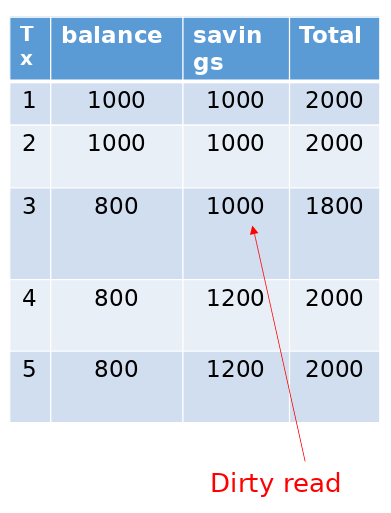
\includegraphics[width=0.25\textwidth]{dirty-reads.png}
    \caption{Dirty read example: every row Tx is the state after a command}
\end{figure}
 

\textbf{Solutions:}

\begin{itemize}
    \item Read locks (=very bad performance)
    \item Remember the old value until commit
    \begin{itemize}
        \item Until the commit happens, every value will be what it was at Tx = 1
    \end{itemize}
\end{itemize}

\subsubsection{Dirty Writes}

\begin{theorem}[Dirty Write]
A dirty write happens when a transaction writes data that has been changed on disk by another transaction. 
The last transaction will overwrite what the first transaction wrote.
\end{theorem}


\begin{figure}[H]
    \centering
    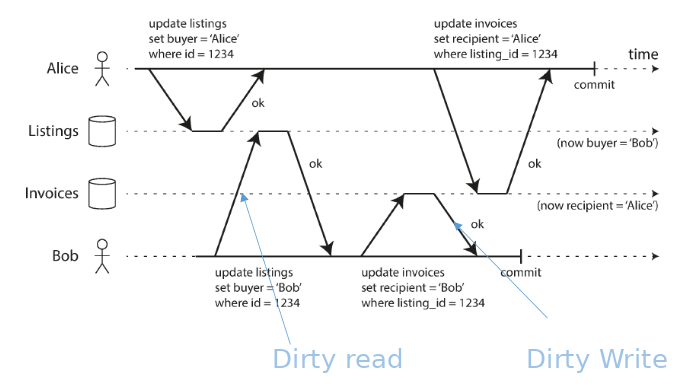
\includegraphics[width=0.6\textwidth]{dirty-reads-lock.png}
    \caption{Dirty write example}
\end{figure}

\begin{enumerate}
    \item Alice buys a car from a dealership
    \item Bob buys the same car from the dealership
    \item Bob gets an invoice before Alice because his internet is faster
    \item Alice gets an invoice after Bob. Two people now own the same car?
\end{enumerate}

\textbf{Solution: Write lock:}

\begin{itemize}
    \item If a row is claimed by a transaction, that row should be locked until commit
    \item Bob cannot write to the invoices, because it has been locked by Alice.
\end{itemize}

\subsubsection{Read skew}

\begin{theorem}[Read skew]
Read skew happens when a commit reads the same data twice, 
with different results because another transaction updated the data.
\end{theorem}

\begin{enumerate}
    \item Alice checks the balance of the first account
    \item Bob updates the balance of the first account
    \item Bob updates the balance of the second account
    \item Alice checks the balance of the second account
\end{enumerate}

Result: Alice `loses' \$100 in one commit, because another transaction changed data.

\begin{figure}[H]
    \centering
    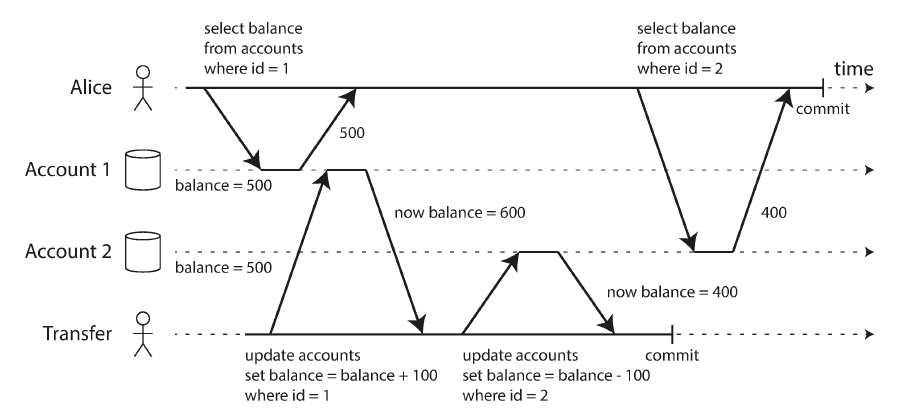
\includegraphics[width=0.6\textwidth]{read-skew.png}
    \caption{Read skew example}
\end{figure}

\textbf{Solution:}

\begin{itemize}
    \item Reading the values again solves the problem
    \item Except for backups: If a backup saves data while another transaction changes it, you will come across problems.
\end{itemize}


\subsubsection{Lost updates \& Atomic updates}

\begin{figure}[H]
    \centering
    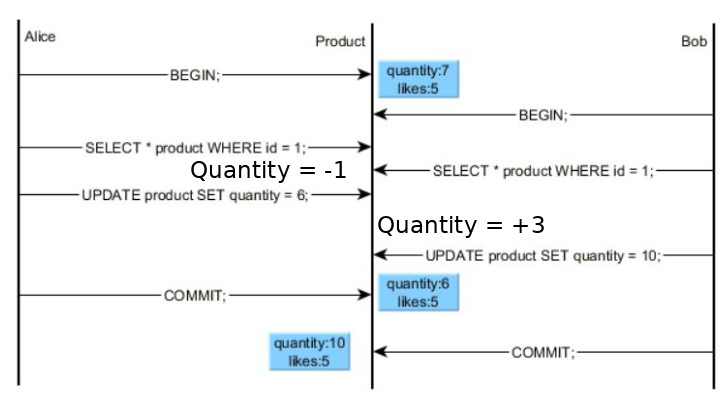
\includegraphics[width=0.5\textwidth]{lost-updates-atomic-updates.png}
    \caption{Lost updates: example}
\end{figure}

\begin{enumerate}
    \item Alice checks the quantity of the product (quantity = 7)
    \item Bob checks the quantity of the product (quantity = 7)
    \item Alice buys the product (quantity = 6)
    \item Bob thinks the quantity is 7 and he wants to add 3: he sets the quantity to 10 (7+3)
    \item Alice commits her changes. According to her, the quantity should be 6
    \item Bob commits his changes. The quantity is 10, overwriting Alice's changes. The actual quantity should be 9 (7-1+3)
\end{enumerate}

\textbf{Solution: Atomic updates}

\begin{itemize}
    \item Problem: Two read - modify - write transactions with different outcomes
    \item Repeatable read does not fix this
    \item Solutions: `atomic updates' or manual lock
    \begin{itemize}
        \item = Exclusive read lock on the data
        \item = No reads or update object until commit
        \item Update `X' SET value = `X2' $\Rightarrow$ (Read - modify - write in one operation)
    \end{itemize}
\end{itemize}

\subsubsection{Write Skew}

Atomic Updates don't protect against everything:

\begin{itemize}
    \item Multi object updates
    \item Lost updates
\end{itemize}

Pattern:

\begin{enumerate}
    \item Read something
    \item Make decision
    \item Write new data
    \item By the time the write is committed, the premise of the decision (step 2) is no longer true, because some other transaction also changed the data
\end{enumerate}

\subsubsection{2-phase lock - Serial execution}

With weak isolation levels:

\begin{itemize}
    \item Readers never block writers
    \item Writers never block readers (you can read the old value while it is being overwritten)
\end{itemize}

With 2-phase lock, there are two fases (duh):

\begin{enumerate}
    \item Exclusive read-lock on data
    \item Exclusive write-lock on data
\end{enumerate}

Problem: \textbf{Deadlocks}

\begin{itemize}
    \item Transactions keep waiting on other transactions' locks
    \item Similar to gridlock: \url{https://en.wikipedia.org/wiki/Gridlock}
    \item Result: the whole database can crash because of this
\end{itemize}

Examples that support 2-phase locking:

\begin{itemize}
    \item MySQL InnoDB
    \item SQL server
    \item DB2 (but DB2 mistakenly calls this `Repeatable read')
\end{itemize}

\subsection{Isolation levels}

= Choose between strong isolation or strong performance

\begin{itemize}
    \item Modern processing 8 - 100+ threads
    \item Choose an isolation level (sorted from weakest to strongest isolation):
    \begin{itemize}
        \item Read Uncommitted (weakest isolation, most performance)
        \item Read Committed
        \item Repeatable Read (=snapshot isolation)
        \item Serial Execution (strongest isolation, least performance)
    \end{itemize}
    \item Isolation problems are hard to debug:
    \begin{itemize}
        \item It's a timing problem
        \item Very hard to reproduce
        \item No errors are logged
    \end{itemize}
\end{itemize}

\begin{figure}[H]
    \centering
    \includegraphics[width=0.7\textwidth]{isolation-levels-dbs.png}
    \caption{(default) isolation levels in current databases. (*) Wrong, Oracle does not comply with ANSI}
\end{figure}


\subsubsection{Isolation level 1: Read Uncommited}

\begin{itemize}
    \item Read Uncommitted offers no protection against concurrency threats
    \item Fastest performance, lowest isolation
    \item One transaction may see not-yet-committed changes made by other transactions
\end{itemize}


\subsubsection{Isolation level 2: Read Committed}

Offers protection against:

\begin{itemize}
    \item Dirty reads
    \item Dirty writes
\end{itemize}

\textbf{Solutions}

\begin{enumerate}
    \item Read locks (bad performance)
    \item Remember the old value until `commit' (better performance)
\end{enumerate}

\subsubsection{Isolation level 3: Repeatable read or Snapshot Isolation}

\begin{itemize}
    \item Also called `Multi Version Concurrency Control (MVCC)'
    \item Solves dirty reads, dirty writes and read skew
    \item If a commit happens before everything is fully backed up, every commit started after the start of the backup will be ignored.
    \item To accomplish this, every transaction gets a number
    \item `Readers do not block writes, writers do not block reads'
\end{itemize}


\subsubsection{Isolation level 4: Serial execution }

\begin{itemize}
    \item One single fast thread (in RAM) for writing
    \item Multiple threads for reading
    \item Not very fast, definitely not very scalable
    \item Only use if your database is not too complex
    \begin{itemize}
        \item Redis
        \item VoltDB
        \item Other databases that can be kept in memory\dots
    \end{itemize}
    \item No write locks necessary, no overhead from thread synchronisation, \dots
    \item Limited by a single thread on your CPU
    \item How to use multiple threads?
    \begin{itemize}
        \item Partition data
        \item Multiple threads, one thread per partition
        \item Speed will be much slower if a transaction accesses multiple partitions
    \end{itemize}
    \item Complete transaction in one serial stored procedure (=piece of code, already compiled and ready to execute)
\end{itemize}

\subsubsection{Conclusion}

\begin{itemize}
    \item Isolation levels are a complex trade-off between\dots:
    \begin{itemize}
        \item Consistency
        \item Scalability
    \end{itemize}
    \item Check your application: which level is the best for your usecase?
    \item 
\end{itemize}


\subsection{ACID: Durable}

= A database should be durable: every write transaction has to be written to disk, and should be stored safely and reliably.

But durability is also a trade-off: 

\begin{itemize}
    \item Higher durability $\Leftrightarrow$ lower performance
    \item Higher performance $\Rightarrow$ more risks
\end{itemize}


\subsubsection{Caching \& BBU}


\begin{itemize}
    \item If we choose the highest isolation on sofware, the hardware can still fail.
    \item For a RAID configuration:
    \begin{itemize}
        \item Most RAID configurations use a RAM cache before writing changes to disks
        \item RAM cache should have a Battery Backup Unit (BBU) in case the power goes out
        \item This is because RAM is by definition not durable, but volatile
    \end{itemize}
    \item Disks also have RAM caches
    \begin{itemize}
        \item This is mostly to sort the data before it gets written
        \item Use professional storage: disks with capacitors!
        \item RAM caches in SSDs have to be Non-Volatile (NV)!
    \end{itemize}
\end{itemize}

\subsubsection{The Transaction chain}

\begin{figure}[H]
    \centering
    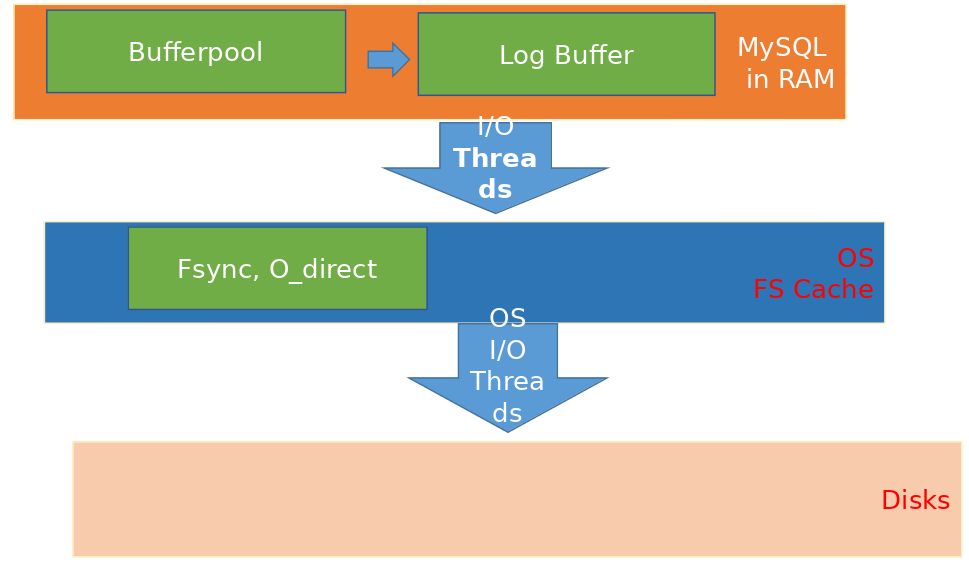
\includegraphics[width=0.5\textwidth]{transaction-chain.png}
    \caption{The transaction chain when writing to disk}
\end{figure}

Steps a transaction takes to write to disk:

\begin{enumerate}
    \item The transaction gets buffered in the buffer pool
    \item The data gets written to the log buffer
    \item Using multiple I/O threads, the log buffer gets flushed to the OS
    \item The OS chooses how the data is written (cache first, or write immediately)
    \item The OS writes the data to the disks
\end{enumerate}

\subsubsection{The transaction chain: innodb\_flush\_log\_at\_trx\_commit}

= a setting in MySQL InnoDB with three options:

\begin{itemize}
    \item 0: Write the log buffer to the log file and flush the log file \textbf{every second}, but do nothing at transaction commits (fastest)
    \begin{itemize}
        \item Fastest
    \end{itemize}
    \item 1: Write the log buffer to the log file and flush it to durable storage \textbf{at transaction commits}
    \begin{itemize}
        \item This is the only option that is fully ACID compliant
        \item It is also the slowest
    \end{itemize}
    \item 2: Write the log buffer to the log file \textbf{at every commit}, but flush it every second
\end{itemize}

\subsubsection{innodb\_flush\_method}

= a setting that tells the OS how the data has to be written

\begin{itemize}
    \item fdatasync
    \begin{itemize}
        \item InnoDB uses fsync() to flush both data and log files (unix)
    \end{itemize}
    \item O\_DIRECT
    \begin{itemize}
        \item This setting still uses fsync() to flush the files to disk, but it instructs the operating system not to cache the data and not to use read-ahead. Avoids double buffering
    \end{itemize}
    \item async\_unbuffered
    \begin{itemize}
        \item Default value on Windows
        \item Causes InnoDB to use unbuffered I/O for most writes
        \item Exception: it uses buffered I/O to the log files when innodb\_flush\_log\_at\_try\_commit = 2
    \end{itemize}
\end{itemize}

\begin{figure}[H]
    \centering
    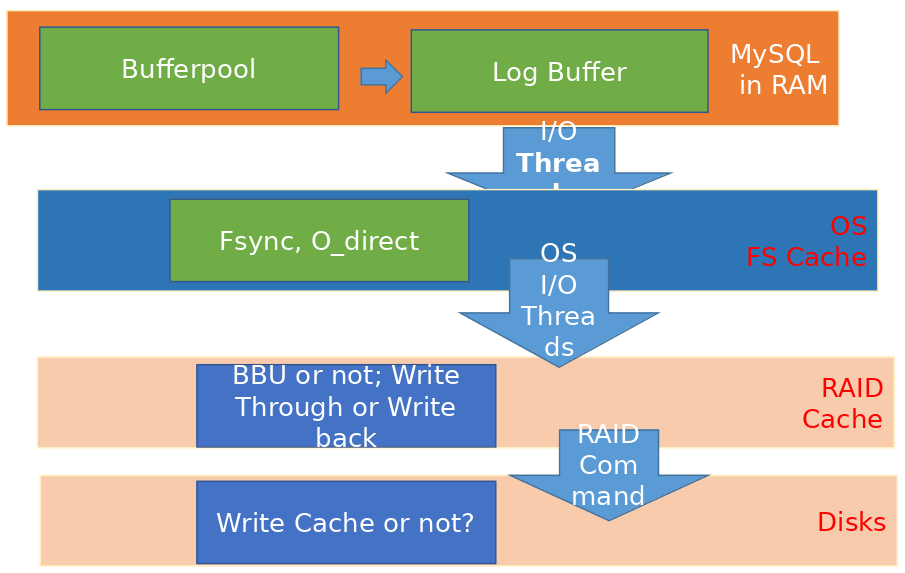
\includegraphics[width=0.5\textwidth]{transaction-chain2.png}
    \caption{The full transaction chain, with RAID}
\end{figure}

\section{NoSQL}

\subsection{SQL}

\subsubsection{Possibilities:}

\begin{itemize}
    \item Relationeel
    \item Column store 
    \item Document store
    \item Graph
    \item Key-value
    \item Specialisten:
    \begin{itemize}
        \item Time series
        \item Text search
    \end{itemize}
\end{itemize}

\begin{figure}[H]
    \centering
    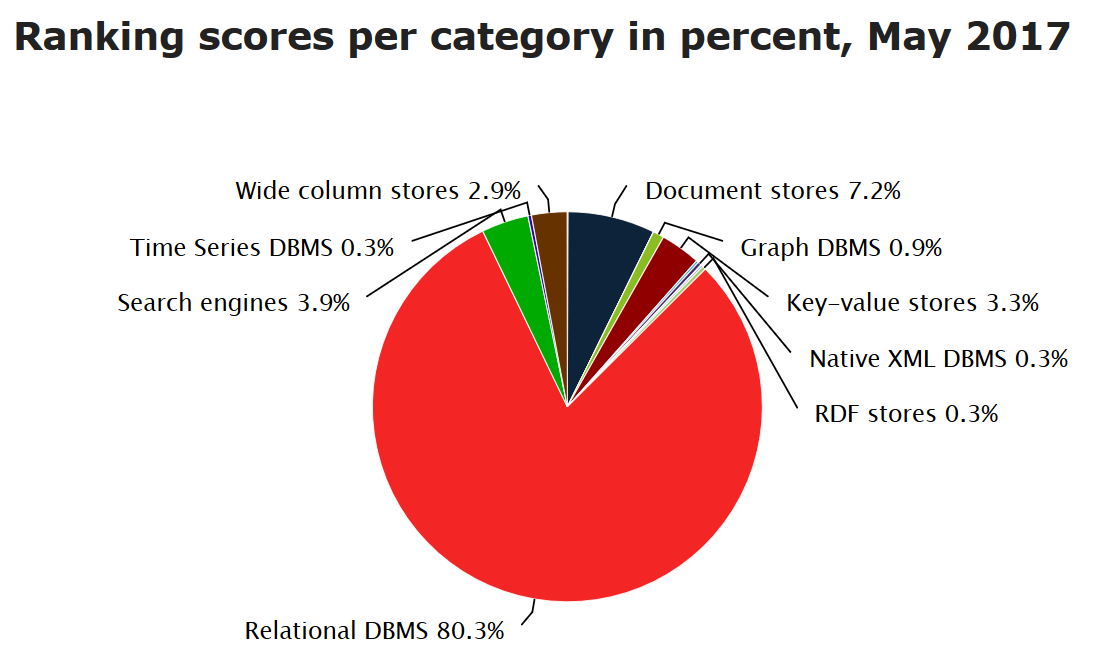
\includegraphics[width=0.5\textwidth]{sql-piechart.png}
    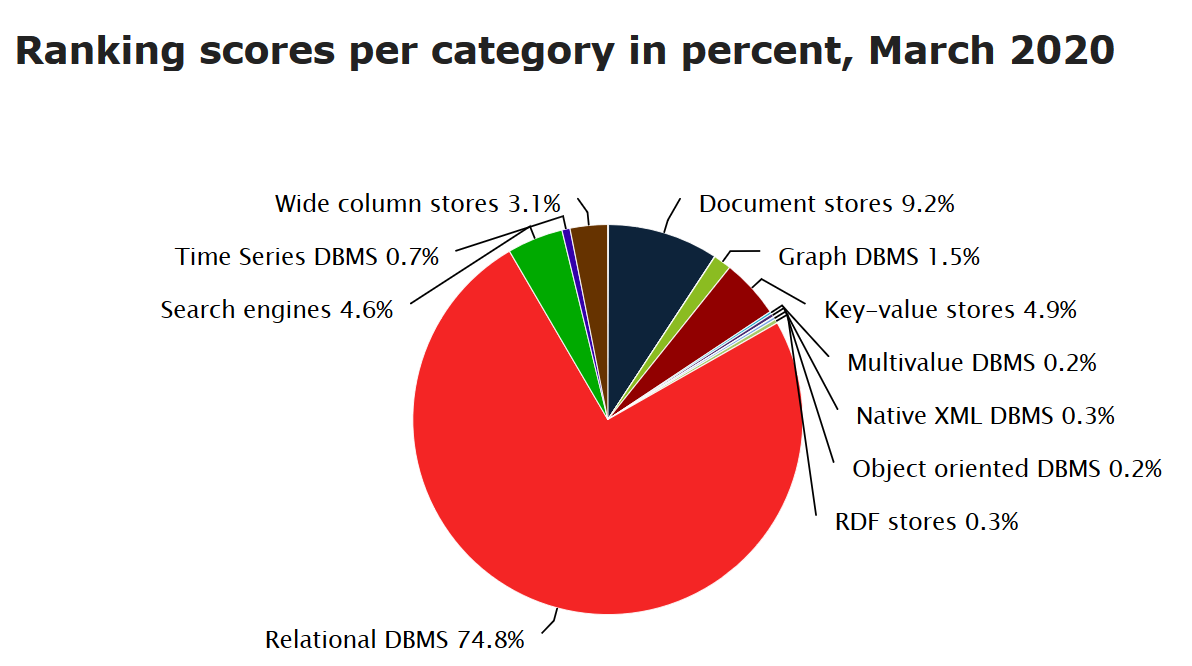
\includegraphics[width=0.5\textwidth]{sql-piechart2.png}
    \caption{Popularity: Relational DBs are the most popular}
\end{figure}

\subsubsection{Imperative languages vs Declarative languages}

\begin{figure}[H]
    \centering
    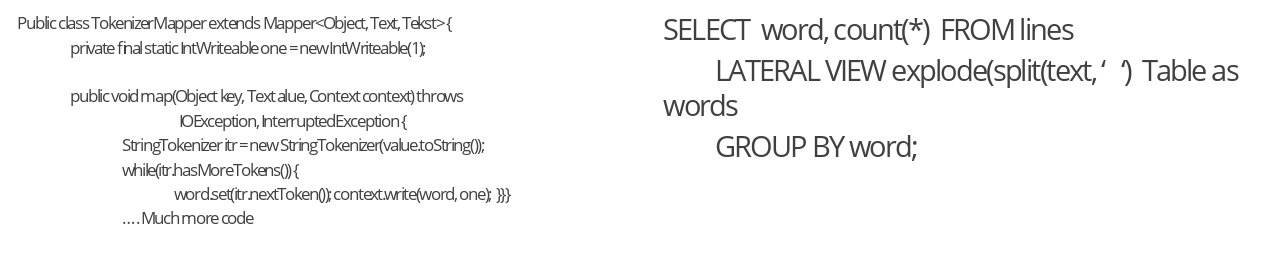
\includegraphics[width=0.8\textwidth]{imperative-vs-declarative.png}
    \caption{Imperative (left) vs Declarative languages (right)}
\end{figure}

\begin{itemize}
    \item Imperative: tell the system how to retrieve/handle/mutate the data, in what order
    \begin{itemize}
        \item C\#, python, \dots
    \end{itemize}
    \item Tell the system the structure of the data you're looking for. Don't tell the system how it has to happen. 
    \begin{itemize}
        \item SQL (uses the query optimizer), HTML + CSS (the browser figures it out)
    \end{itemize}
\end{itemize}

\subsection{B-tree index}

\subsubsection{Index}

Index of a book:

\begin{itemize}
    \item Summary/copy that allows to search faster in the main structure (book/database)
    \item Redundant (copy), needs disk space (needs `pages')
\end{itemize}

Index of a database:

\begin{theorem}[Index]
    A copy of some columns from a table, sorted, that improves the speed of data retrievel operations at the cost of additional writes and storage space.
    Indexes are used to quickly locate data without having to search every row in the database.
\end{theorem}

\begin{itemize}
    \item \url{https://en.wikipedia.org/wiki/Database_index}
    \item \url{https://use-the-index-luke.com/sql/anatomy}
\end{itemize}

\subsubsection{B-tree index}

\begin{theorem}
    A B-tree index stands for `balanced tree index' and is a type of index that can be created in relational databases.
    It works by creating a series of nodes in a hierarchy. The nodes cover a range of values of row IDs. 
    It’s called a tree because it has a root, several branches, and many leaves.
    
    The leaves make up a doubly linked list: \url{https://en.wikipedia.org/wiki/Doubly_linked_list}
    
\end{theorem}

\begin{figure}[H]
    \centering
    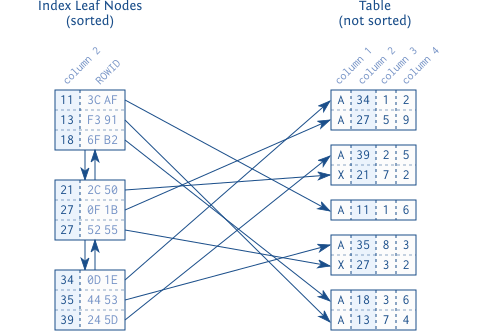
\includegraphics[width=0.6\textwidth]{b-tree-index.png}
    \caption{}
\end{figure}

\begin{itemize}
    \item The leaf nodes make up a doubly linked list
    \begin{itemize}
        \item Every block refers to other blocks: the next and previous block
        \item Every block has key-value items: Index + Row ID (or index + value in `key value' DBs)
        \item Insert = add new links to the list
    \end{itemize}
    \item This index is stored in RAM:
    \begin{itemize}
        \item If you have to jump from one block to another block, sequential disks are too slow for random access: random read/writes are much faster with RAM
        \item If you have 10 million records: serial search is way too slow!
    \end{itemize}
\end{itemize}

\subsubsection{Tree architecture}

\begin{figure}[H]
    \centering
    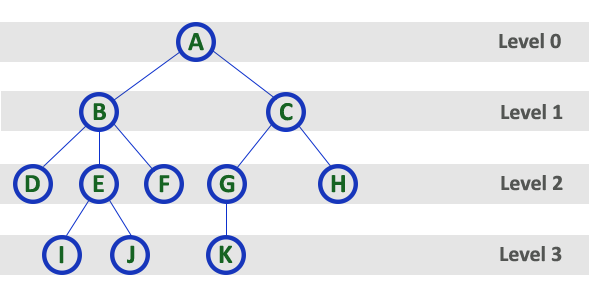
\includegraphics[width=0.5\textwidth]{tree-architecture.png}
    \caption{A balanced tree}
\end{figure}

\begin{itemize}
    \item A = root
    \item B \& C = child (pages)
    \item AC = edge
    \item Depth A to K = 3 (=amount of edges)
    \begin{itemize}
        \item From root to leaf
    \end{itemize}
    \item I, J, K = leaf nodes (point to data)
\end{itemize}

\subsubsection{Searching for an index}

\begin{figure}[H]
    \centering
    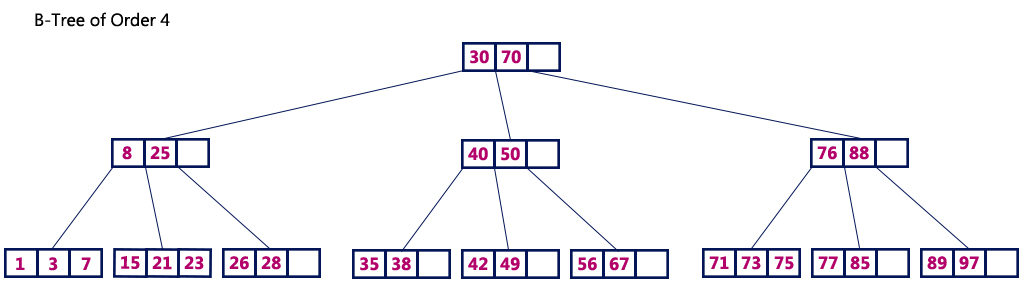
\includegraphics[width=0.7\textwidth]{balanced-tree-index.png}
    \caption{Balanced tree example: how do you find index 38?}
\end{figure}

\begin{enumerate}
    \item Start at the root node and search from node 30
    \item Go to the next level and find node 40
    \item Search from node 35 (depth 3), now read serially
    \item Find row id in index 38
\end{enumerate}

\subsubsection{Size}

\begin{itemize}
    \item Block size = 16KB
    \item Branching factor = 100 (=number of children for each node)
    \item Depth = 3
    \item $100 \cdot 100 \cdot 100 \cdot 16\text{KB} = 16\text{GB}$
    \begin{itemize}
        \item Typical depth: 4
        \item Typical branches = 100s
    \end{itemize}
\end{itemize}

\subsubsection{B-trees: getting faster \& more reliable}

\begin{theorem}[WAL]
    A Write Ahead Log is a type of file (you can also call it a type of sequential database) where database changes are first recorded (append-only).
    These changes must be written to stable storage, before the changes are reliably written to the database.

    Another name for WAL is a redo log: each log file consists of redo records. A redo record holds a group of change vectors, each of which represents a change made to a single block in the database
\end{theorem}

\begin{itemize}
    \item 1 Update = 2 writes: when data gets updated, the index also needs to get updated:
    \begin{enumerate}
        \item Update the WAL or REDO log
        \item Page update
    \end{enumerate}
    \item If something fails when it's updating the page, the DB will try again using the data in the WAL/REDO log
    \item Less levels vs more branches:
    \begin{itemize}
        \item Each level can be a disk seek
        \item Using more branches means less disk seeks
    \end{itemize}
\end{itemize}


\subsubsection{Dataminded: Python + Postgres}

Dataminded = consultent in big data technology with lots of experience using big data tools.

But: Python + Postgres can handle almost any analytics challenge

\begin{figure}[H]
    \centering
    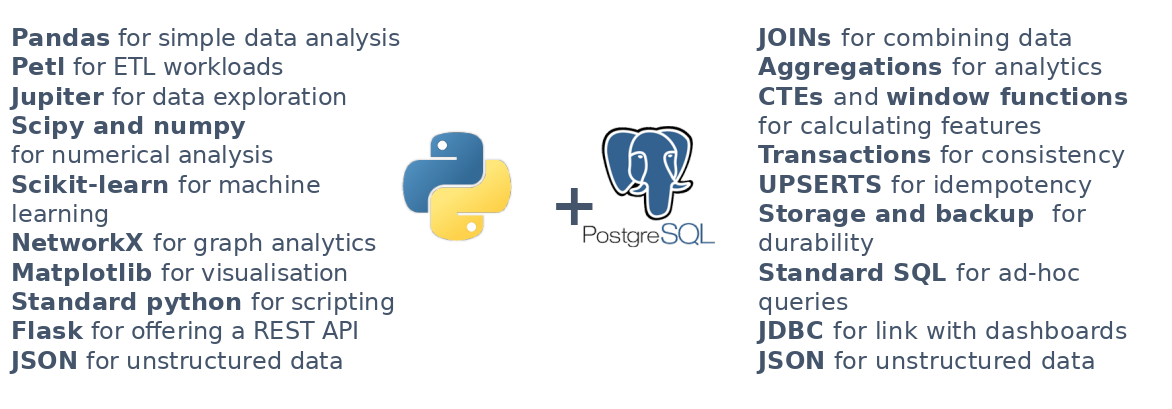
\includegraphics[width=0.5\textwidth]{python-postgres.png}
    \caption{Use python libraries + a relational database for most analytics}
\end{figure}

\subsubsection{When is SQL not the answer}

\begin{itemize}
    \item \textbf{Volume} = When you have petabytes of data (rare)
    \item \textbf{Velocity} = Too many writes per second (less rare)
    \item \textbf{Scalability}
    \begin{itemize}
        \item Want to avoid expensive servers
        \item Want to avoid expensive SANs (Storage Area Networks)
    \end{itemize}
    \item \textbf{Variety} = When you don't want to turn an object (with unstructured data) into a relational row
    \begin{itemize}
        \item = Object - relational database mismatch
        \item \url{https://en.wikipedia.org/wiki/Object%E2%80%93relational_impedance_mismatch}
    \end{itemize}
\end{itemize}

\subsection{Key-Value}

\begin{itemize}
    \item Key-value DBs are relatively simple databases
    \item Adding to the end of a file is the fastest way to write
    \item Example: a list of videos with their watch time
    \begin{itemize}
        \item Key =  video ID
        \item Value = watch time, gets incremented often
    \end{itemize}
\end{itemize}

\subsubsection{Hash index}

= a hashed key that will be searched for

\begin{itemize}
    \item the hash (stored in RAM) will point to an offset on the disk
    \item if you find the key, you'll find where on the disk the data is stored
    \item if you want to update data, it will get appended to the end (=segment 2)
\end{itemize}

\begin{figure}[H]
    \centering
    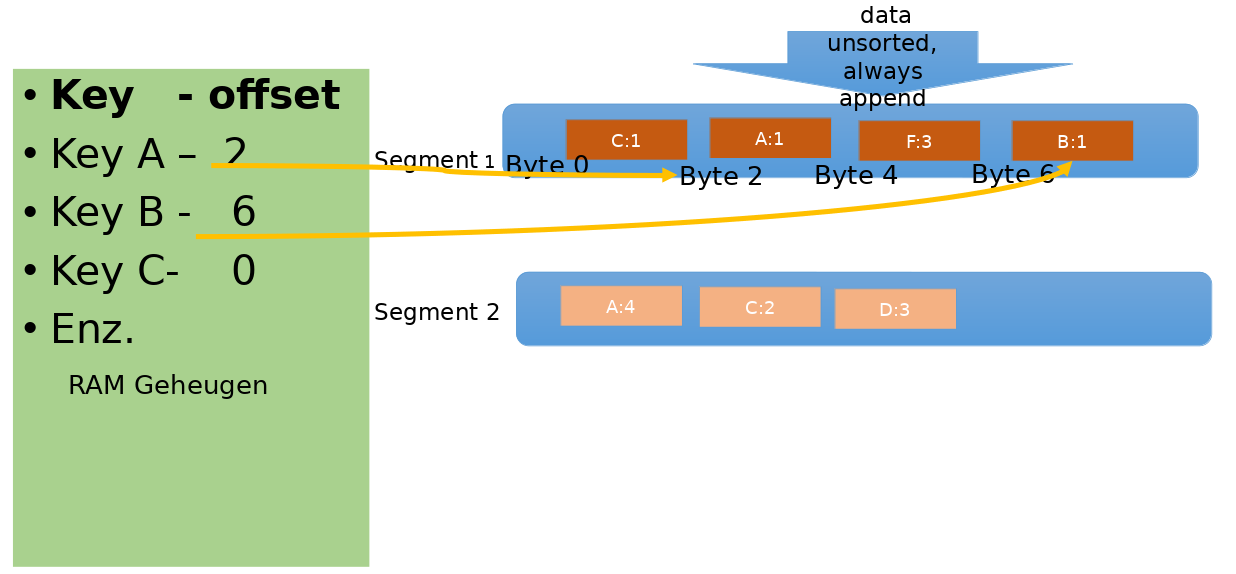
\includegraphics[width=0.5\textwidth]{key-value.png}
    \caption{Log structure + hash index}
\end{figure}

\subsubsection{Compacting}

\begin{figure}[H]
    \centering
    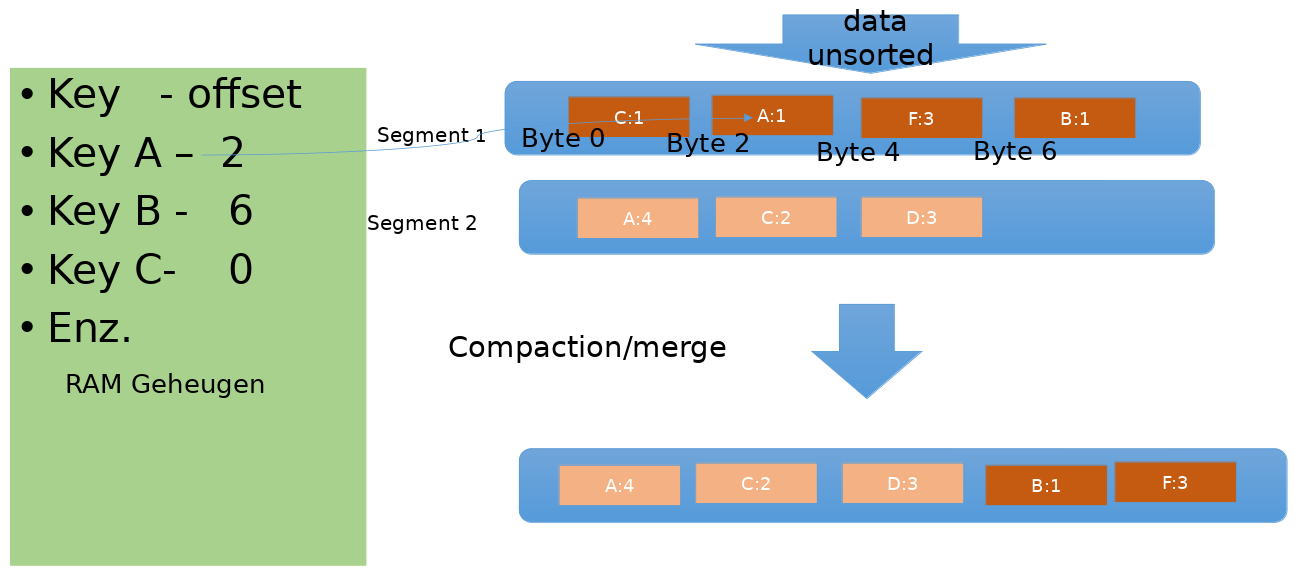
\includegraphics[width=0.5\textwidth]{key-value-compacting.png}
    \caption{Compaction/merge of 2 segments}
\end{figure}

\begin{itemize}
    \item In the above example: $A = 1$ in segment $1$, but $A = 4$ in segment $2$
    \item Segment $2$ is newer: we ignore the first segment's $A$
    \item Same for $C$ ($C=1 >> C=2$)
    \item We compact/merge the segments until stored the data is correct
    \item We do this often
\end{itemize}

\subsubsection{Principles}

\begin{itemize}
    \item Very fast writes (append only, so you can write sequentially because disks won't need to change tracks)
    \item Very fast reads if (sorted) hash index is in RAM
    \begin{itemize}
        \item if not: very slow
        \item SELECT * FROM A TO ZZZ (=slow)
    \end{itemize}
    \item On crash: no corruption because of wrong update
    \item Example key-value hash index: Riak Bitcask (\url{https://en.wikipedia.org/wiki/Riak})
\end{itemize}

\subsection{LSM: Log Structured Merge Tree}

Apart from the hash index, there is another Log Structured data store: the \textbf{Log Structured Merge Tree} with \textbf{Sorted String tables}

\begin{itemize}
    \item Unsorted data now gets sorted first in a memory buffer (RAM)
    \begin{itemize}
        \item Log segment file as backup
    \end{itemize}
    \item Then it gets written to a segment
    \item Just like a hash index: values are not updated, but appended in a new segment
    \item Write to disk after several MB (to sorted string table file)
\end{itemize}

\begin{figure}[H]
    \centering
    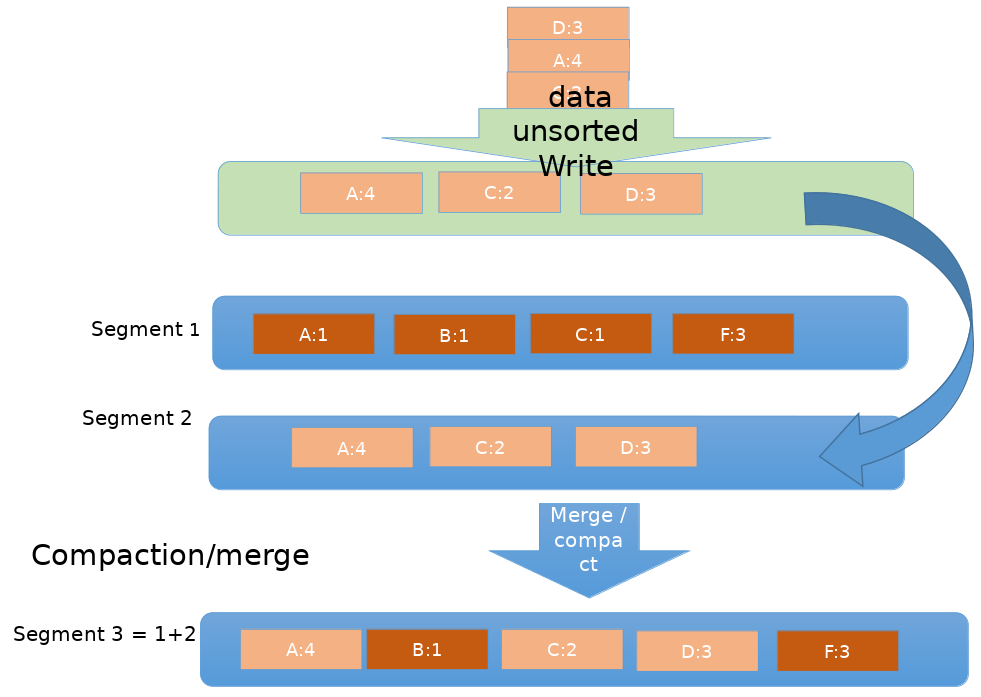
\includegraphics[width=0.6\textwidth]{lsm.png}
\end{figure}


\subsubsection{Log Structure Merge + Sparse tree index}

\begin{figure}[H]
    \centering
    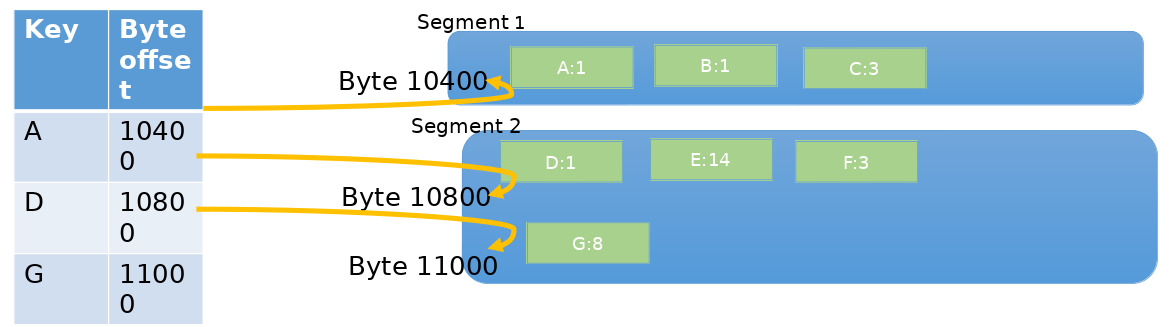
\includegraphics[width=0.6\textwidth]{lsm-sparse-tree-index.png}
    \caption{Sparse tree index}
\end{figure}


\begin{itemize}
    \item We can simplify the LSM
    \item You don't need to keep every key in RAM
    \item Sparse tree index $\Rightarrow$ remember where some milestones are
    \begin{itemize}
        \item If you need F, and you know where D and G are
        \item Start reading from D (byte-offset 10800)
        \item Read sequentially until G (byte-offset 11000)
        \item This sequential read is very quick, because it's a small amount of keys
    \end{itemize}
    \item Merge, compact \& sort every time = string sorted table
    \item Every delete: create new segment and merge. 
    \item `Tombstone the old segment' = marking key/value pairs for deletion
\end{itemize}

\subsubsection{Applications of Sorted String \& LSM-tree}

\begin{itemize}
    \item First application: Google Big Table (\url{https://en.wikipedia.org/wiki/Bigtable})
    \item LevelDB (also by Google), RocksDB (fork of LevelDB)
    \item MyRocks (=a RocksDB storage engine for MySQL)
    \item Hbase, Cassandra (Facebook)
    \item ElasticSearch: based on Lucene text search (key = text, value = document) or inverted index
\end{itemize}

\subsubsection{Advantages LSM}

\begin{itemize}
    \item Very fast writes (append-only)
    \item Quite fast reads (sparse index)
    \item Easily scaled over nodes (segments)
\end{itemize}

\subsubsection{Disadvantages LSM}

\begin{itemize}
    \item Write (merge \& delete) in background can influence speeds
    \item Deletes are costly because you don't actually delete: you tombstone a segment (=mark for deletion, it only gets deleted at the compaction step)
    \item You have to specify the rate between compaction \& write/read (ongoing action) yourself
\end{itemize}

\subsubsection{Summary: B-Trees vs LSM trees}

Explain:

\begin{itemize}
    \item Why do Write-Ahead Logs (WAL) exist?
    \item What is a compactor? Compaction planning?
    \item Advantages \& disadvantages with much or little compacting?
\end{itemize}

\subsection{Time Series}

= LSM with a twist

\begin{figure}[H]
    \centering
    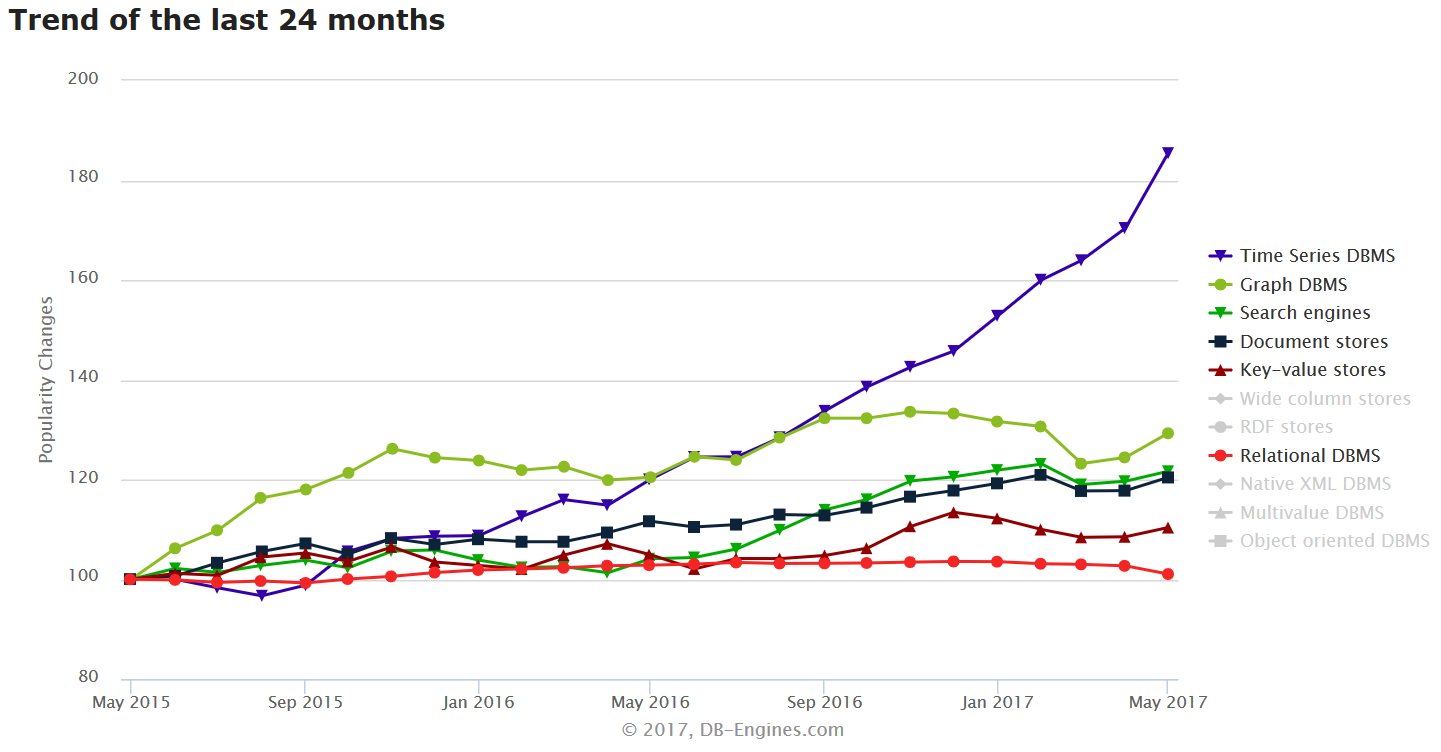
\includegraphics[width=0.5\textwidth]{time-series-lsm.png}
    \caption{Popularity time series}
\end{figure}

Why the sudden rise in popularity?

\begin{itemize}
    \item IoT devices use lots of sensors that need to be logged
    \item That sensor data is time based
\end{itemize}

\subsubsection{Properties}

\begin{itemize}
    \item Lots of individual data points: `a row is not important'
    \begin{itemize}
        \item If you lose a data point, that's not a problem
        \item You can guess what the data point would be, based on the data around the same timeframe
    \end{itemize}
    \item High write throughput
    \item High read throughput (aggregation per hour/day)
    \item Large deletes (data expiration)
    \item Mostly an insert/append workload, very few updates
\end{itemize}

\subsubsection{Use case: windmill sensors}

Situation: a windmill has many sensors that produce data that needs to be logged

\begin{itemize}
    \item Turbine sensor data needs to be stored every second
    \begin{itemize}
        \item 30 sensor readings per second
        \item > 300GB per windmill per year
    \end{itemize}
    \item Both aggregation and realtime
    \item Issue with MySQL databases: read locks during queries $\Rightarrow$ INSERT fails $\Rightarrow$ causing data loss
\end{itemize}

\subsubsection{Case study: influx DB}

\url{https://docs.influxdata.com/influxdb/v1.4/concepts/storage_engine/}

Exercise: `read the entire page, understand everything, and answer these questions:'

\begin{itemize}
    \item Why important for MCT?
    \item How can you scale?
    \item TSM?
    \item WAL? How durable? What is it?
    \item What is a compactor? Compaction planning?
    \item Give one example of unique functionality typical for a time series environment
    \begin{itemize}
        \item Tip: say you need to aggregate every hour
    \end{itemize}
\end{itemize}

\subsubsection{Object - relational mismatch}

\begin{theorem}
    Object-relational mismatch is a set of technical difficulties that are often
    encountered when an RDBMS is being served by an application program written 
    in an object-oriented programming language, because objects or class definitions 
    must be mapped to database tables defined by a relational schema.
\end{theorem}

\begin{figure}[H]
    \centering
    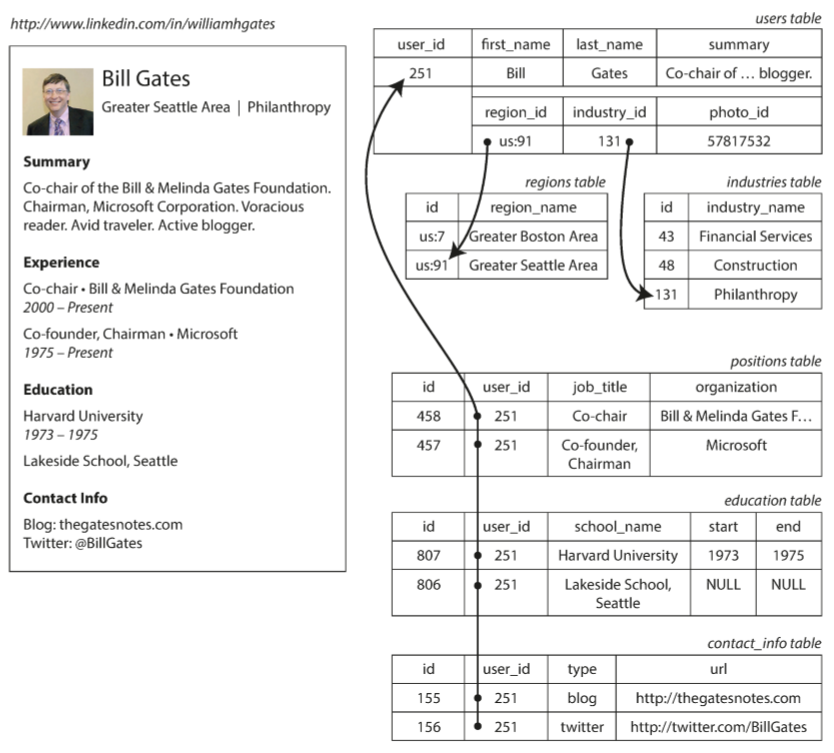
\includegraphics[width=0.5\textwidth]{billgates.png}
    \caption{Representing an object in relational rows}
\end{figure}

\begin{itemize}
    \item Example: a LinkedIn-like application on an RDBMS with lots of 1 to n relations
    \item These relations are prone to object-relational mismatch problems
    \item A better match for objects with unstructured 1-n data: JSON documents:
\end{itemize}

\begin{minted}{json}
{
    "user_id": 251,
    "first_name": "Bill",
    "last_name": "Gates",
    "positions": [
        {"job_title": "Co-chair", "organization": "Bill & Melinda Gates Foundation"},
        {"job_title": "Co-founder, Chairman", "organization": "Microsoft"}
    ]
}
\end{minted}

\subsubsection{JSON in PostgreSQL}

\begin{itemize}
    \item Mid 2014: PostgreSQL 9.4 natively supports JSON
    \item The speed to ingest documents as quickly as MongoDB, but ACID!
    \item Fully indexable
\end{itemize}

\subsection{ElasticSearch}

\begin{itemize}
    \item = a document Store
    \begin{itemize}
        \item So naturally suited for describing objects
        \item JSON serialized
    \end{itemize}
    \item Easy access to an advanced fulltext search-engine library
    \item Lucene is very complex but very advanced
    \begin{itemize}
        \item Lucine = LSM sorted string table that works with segments
        \item Automatized sharding (and thus scalable) in containers
    \end{itemize}
    \item Has a RESTful API: you can use commands like curl, wget, \dots to interact with the database as if it's a website
    \item Data ingest is not very fast (`index')
    \begin{itemize}
        \item Can be used for time series, but a real time series DB is better
    \end{itemize}
\end{itemize}

\subsubsection{Elastic Search architecture, the basics}

\begin{itemize}
    \item Document = JSON data
    \item Index = a collection of documents (ElasticSearch index $!=$ database index)
    \item Shards = scalable pieces of index
    \item Segments = sequential pieces of a shard
\end{itemize}

\begin{figure}[H]
    \centering
    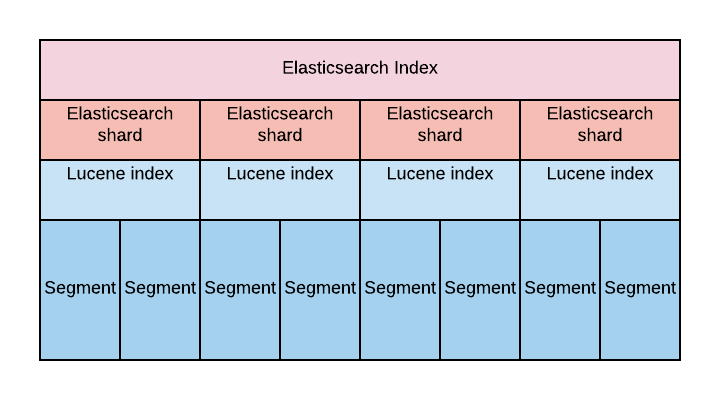
\includegraphics[width=0.6\textwidth]{elasticsearch-architecture.png}
    \caption{Elastic Search architecture}
\end{figure}

\subsubsection{Elastic Search Cluster}

\begin{itemize}
    \item Index is split over shards - nodes: scalability
    \item Shards can be replicated over nodes: availability
\end{itemize}

\begin{figure}[H]
    \centering
    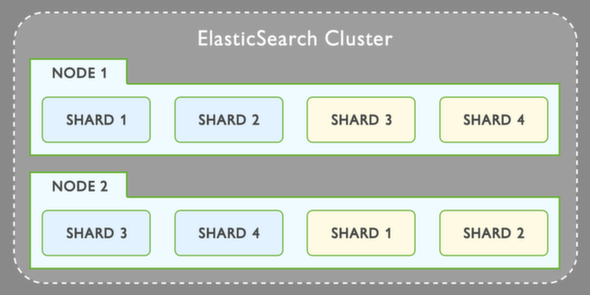
\includegraphics[width=0.5\textwidth]{elasticsearch-searchcluster.png}
\end{figure}

\subsubsection{Inverted index}

\begin{theorem}
    An inverted index is a database index storing a mapping from content, such as words or numbers, to its locations in a table or document.

    This is in contrast to a `forward index', which maps from documents to content.
\end{theorem}

\begin{itemize}
    \item The power of ElasticSearch is text search using Lucine
    \item = `Lucene Index'
    \item A document will be seen as important if it contains a relevant word many times
    \item If a word is very common, Lucine will see it as a stopword (a, and, for, is, in, it, \dots)
    \item Lucine can work with misspelled words, using a certain `distance' of characters (= amount of characters that can be wrong)
    \item Disadvantage: increased processing when a document is added to the database
\end{itemize}

\begin{figure}[H]
    \centering
    \includegraphics[width=0.7\textwidth]{inverted-index.png}
    \caption{Inverted index: an index where words are mapped to the location where that word appears}
\end{figure}

\subsubsection{GeoHashes: Representing Geospatial data in ElasticSearch}

\begin{figure}[H]
    \centering
    \includegraphics[width=0.5\textwidth]{geohashes.jpg}
\end{figure}

How it works is less important for this module, just know that it exists and uses ElasticSearch's text search capabilities

\begin{itemize}
    \item Since ElasticSearch 0.90
    \item Base32 encoded strings, interleaving the latitude and longitude
    \item Max resolution: 40mm * 20mm
    \item Each extra symbol divides the grid in 26 cells
\end{itemize}

\subsubsection{ElasticSearch scaling}

\begin{figure}[H]
    \centering
    \includegraphics[width=0.5\textwidth]{elasticsearch-scaling.png}
\end{figure}

\begin{itemize}
    \item ElasticSearch is very scalable
    \item 1 node $\Rightarrow$ 2 nodes: almost double the performance
\end{itemize}

\subsection{Which storage engine is the best and the worst}

Which storage engine is the best/worst for the following situations:

\begin{itemize}
    \item High amount of writes every second (sensor data)
    \item High amount of updates every second: Web analysis data (Marketing campaign)
    \item Continuous updates and reads of personal data? 
    \item Full scans on structured data?
    \item ACID compliant OLTP?
\end{itemize}

\subsection{Summary}

\subsubsection{Hash index vs LSM datastore}

\textbf{Hash index}

\begin{itemize}
    \item Fast reads when index is in RAM
    \item Very fast writes (append)
    \item Slow scans (select *, group by, \dots)
\end{itemize}

\textbf{Log Structured Merge Tree}

\begin{itemize}
    \item Fast read speed (offset + sequential scan), \textbf{a bit slower than hash index}
    \item Very fast writes (append)
    \begin{itemize}
        \item But because of sorting in RAM, we need to first write to a read-ahead log
        \item Or else data can be lost if the data is still being sorted in the memory buffer (for example due to power failure)
    \end{itemize}
    \item \textbf{Fast scans} because of sorted string tables
\end{itemize}

\subsubsection{B-tree vs LSM}

\textbf{B-tree}

\begin{itemize}
    \item \textbf{Very} fast in random reads
    \item \textbf{Fast updates}
    \item Not useful for high volume writes
    \item Very fast scans when index is on correct column
\end{itemize}

\textbf{LSM Tree}

\begin{itemize}
    \item Fast read speeds
    \item Slower in updates because of tombstone: mark for delete + append
    \item \textbf{Very fast writes} (append)
    \item Very fast scans (sorted!)
\end{itemize}

\section{Distributed Stores}

\begin{theorem}
    A distributed data store is a computer network where information is stored on 
    more than one node, often in a replicated fashion.

    It is the perfect match for big data: volume, velocity, variety
\end{theorem}

\subsection{Terminology}

\subsubsection{Shard/partition}

\begin{theorem}
    A shard or partition is a small subset of the database that can be assigned to a node
\end{theorem}

\begin{itemize}
    \item The database is divided into nodes
    \item ElasticSearch, MongoDB, MySQL: `Shard'
    \item Hbase: `Region'
    \item Cassandra, Riak: `vnode'
\end{itemize}

\subsubsection{Replica}

\begin{theorem}
    A replica is a copy of a shard/database that is kept on a different machine
\end{theorem}

\begin{itemize}
    \item If a shard gets corrupted or lost, replicas serve as a backup solution
    \item The replicas are kept on \textbf{different} nodes: never on the same node
\end{itemize}

\begin{figure}[H]
    \centering
    \includegraphics[width=0.5\textwidth]{partitions-replicas-nodes.png}
    \caption{Shards and Replicas are split over multiple nodes}
\end{figure}

\subsection{Elastic Search Cluster}

\begin{figure}[H]
    \centering
    \includegraphics[width=0.5\textwidth]{elasticsearch-cluster.png}
    \caption{Example cluster with 2 nodes, 1 replica shard for each node}
\end{figure}

\begin{itemize}
    \item Index is split over shards - nodes: \textbf{Scalability}
    \item Shards can be replicated over nodes: \textbf{Availability}
\end{itemize}

\subsection{Replication: master/slave or leader/follower}

\begin{figure}[H]
    \centering
    \includegraphics[width=0.4\textwidth]{replication-master-slave.png}
    \caption{}
\end{figure}

\begin{itemize}
    \item Multi-node or distributed data systems can be quite complex
    \item The master (one server) does all read and write operations
    \item The data gets copied to the slave (the replica) for redundancy
    \item You can only read to the slave 
\end{itemize}

\subsubsection{Communication between master \& slave, two ways:}

\textbf{Synchronously}

\begin{itemize}
    \item The master writes new data to the slave
    \item The slave must acknowledge the data
    \item The master must wait for the confirmation by the slave
    \item Consistent data
    \item Slow \& unreliable with many slaves
\end{itemize}

\textbf{Asynchronously}

\begin{itemize}
    \item No acknowledgment of slave
    \item Inconsistent data
    \item Fast, even with many slaves
\end{itemize}

\subsubsection{Consistency choices}

\textbf{Strong Consistency}

\begin{itemize}
    \item At a certain point in time after a write, all replicas return the same update record/document (almost realtime)
    \item Consistent with order in which write operations are submitted by clients
\end{itemize}

\textbf{Eventual Consistency + High availability}

\begin{itemize}
    \item Faster, easier to be `available'
    \item Hard for devs: when updating a row, you can not be sure when it will be updated in other nodes
    \item Every request received by a non-failing node must result in a `non-error' response
    \item Nodes can read/write - even if that means that not all replicas have the same content
\end{itemize}

\subsubsection{Amount of leaders}

\textbf{Single leader}

\begin{itemize}
    \item Only one node (the leader) can write
    \item The follower gets the updates as fast as possible, synchronously
    \item Only for systems with few write operations and many read operations
    \item Strong consistency is possible
\end{itemize}

\textbf{Multi leader}
\begin{figure}[H]
    \centering
    \includegraphics[width=0.35\textwidth]{replication-multi-leader.png}
    \caption{Multi leader}
\end{figure}

\begin{itemize}
    \item More than one node can write
    \item $\Rightarrow$ write conflicts are possible, because the same data can be updated on different nodes
    \item These conflicts must be solved $\Rightarrow$ system is much more complex
    \item Not consistent = replica may be out of sync
\end{itemize}

\subsubsection{Split-brain and Network partition}

\begin{theorem}
    Network partitioning happens when a network is split due to the failure of network devices.
    The network devices stop communicating and synchronizing their data to each other.
\end{theorem}

\begin{theorem}
    Split-brain is a problem that indicates data or availability inconsistencies
    originating from the maintenance of two separate data sets, for example because
    of network partitioning.
\end{theorem}

What if the network connection drops?

\begin{itemize}
    \item Do we allow the follower to become the leader?
    \item Or do we block from writing to follower?
    \item But leader might still be alive and serving
    \item Result: if we allow data to be written to the follower, and the leader is still serving, both nodes might have different data
\end{itemize}

\subsection{CAP Theorem}

\begin{theorem}
    The CAP theorem states that it is impossible for a distributed data store to 
    simultaneously provide more than two out of the following three guarantees: 

\begin{itemize}
    \item \textbf{Consistency}: every (later) read operation will always return the last version (*) of the data, or an error message (single object)
    \begin{itemize}
        \item (*): last written by a write operation X older than this read operation
    \end{itemize}
    \item \textbf{Availability:} there is always a server available, if necessary: with older data
    \item \textbf{PartitionTolerance:} the system must keep working, even if the nodes can't communicate with each other (`network partitioning')
\end{itemize}
\end{theorem}

We can use the CAP theorem to describe the problems originating from network partitioning.


\begin{figure}[H]
    \centering
    \includegraphics[width=0.9\textwidth]{cap-theoreum.png}
    \caption{Oversimplification of CAP theorem}
\end{figure}

\subsubsection{CAP: either consistent or available when partitioned}

\begin{itemize}
    \item When we come accross network partitioning, we will have to choose between 2 properties if we want to keep partition tolerance:
    \begin{itemize}
        \item Consistency
        \item Availability
    \end{itemize}
    \item Both at the same time is NOT possible
    \item When there is no network partitioning, then both Consistency and Availability are satisfied
\end{itemize}

$\Rightarrow$ We will look at a couple possible situations, using a relational database as an example:

\subsubsection{Relational DB: CA}

\begin{figure}[H]
    \centering
    \includegraphics[width=0.3\textwidth]{cap-theorem-ca.png}
\end{figure}

\begin{itemize}
    \item If we want to keep consistency, we will only allow reads to the slave
    \item Only consistent if perfectly synchronized
    \item In reality, we only allow reads to slave
    \begin{itemize}
        \item $\Rightarrow$ no `A' for writes
        \item $\Rightarrow$ CAP theorem has no value here
    \end{itemize}
\end{itemize}


\subsubsection{Relational DB: CA: single node (no P possible)}

\begin{figure}[H]
    \centering
    \includegraphics[width=0.4\textwidth]{cap-theorem-ca-single.png}
\end{figure}

\begin{itemize}
    \item = simpler system: single node: we only read / write to one node
    \item Partition tolerance is not possible because there is no network between nodes
    \item $\Rightarrow$ CAP theorem also has no value here
\end{itemize}

\subsubsection{AP systems}

\begin{figure}[H]
    \centering
    \includegraphics[width=0.6\textwidth]{cap-theorem-ap.png}
    \caption{AP: ensure Availability and PartitionTolerance when there is network partitioning}
\end{figure}

\begin{itemize}
    \item The system will always return data, but not always consistent (if network issues between nodes)
    \item If we read or write data and this fails, another node will take control, no error messages
    \item We choose AP in situations where reading data is more important than writing
    \item But how available is this system in reality?
    \begin{itemize}
        \item It might take a while before replica's know they can't synchronize
        \item There might be considerable lag when waiting for a response
        \item $\Rightarrow$ not as much availability after all $\Rightarrow$ not so useful
    \end{itemize}
\end{itemize}


\subsubsection{CP}

\begin{figure}[H]
    \centering
    \includegraphics[width=0.5\textwidth]{cap-theorem-cp.png}
    \caption{Consistency and PartitionTolerance: The system will always return the correct data}
\end{figure}

\begin{itemize}
    \item When network partitioning happens, consistency is kept: it will either not return data, or return the correct data
    \item We will not be able to read the data as long as these were not written to all nodes
    \item If we can't write data, we will see an error message $\Rightarrow$ no availability
    \item We can use CP if data consistency is very important
\end{itemize}


\subsubsection{Conclusion 1}

CAP theorem is not clear way to make architectural choices. The creators even admitted this.

\begin{itemize}
    \item CA doesn't exist: >1 node \& partitioning == no real availabilty anymore (only for read)
    \item When CAP theorem describes consistency, it talks about a single object, but in many applications consistency over many rows (in many tables) is important
    \item No CP: with many replicas, you should choose for asynchronous replication:
    \begin{itemize}
        \item So no strong consistency
        \item No availability (no writes possible)
    \end{itemize}
\end{itemize}

\subsubsection{Conclusion 2}

CAP theorem only serves to clarify the difference between AP vs Single node consistency

\begin{itemize}
    \item When using multiple nodes, there is only `eventual consistency' and `read availability' $\Rightarrow$ CP is impossible
    \item Multi node systems are always a little inconsistent
    \item AP is possible but only for partition problems
    \begin{itemize}
        \item Is being available in 1 situation (network partition, rare) even that useful?
    \end{itemize}
\end{itemize}

\subsection{How does Elastic Search handle network partitioning?}

\subsubsection{Consistency and Network partitioning}

\url{https://www.elastic.co/guide/en/elasticsearch/reference/2.4/docs-index\_.html#index-consistency}

\begin{itemize}
    \item To prevent writes from taking place on the `wrong' side of a network partition
    \item By default, index operations only succeed if a quorum(=voting procedure) (>replicas/2+1) of active shards are available. 
    \item This default can be overridden on a node-by-node basis using the action.write\_consistency setting. 
    \item To alter this behavior per-operation, the consistency request parameter can be used.
    \item Valid write consistency values are one, quorum, and all.
\end{itemize}


\begin{figure}[H]
    \centering
    \includegraphics[width=0.5\textwidth]{elasticsearch-distributed.png}
    \caption{ElasticSearch }
\end{figure}

\begin{itemize}
    \item In the above example: we have 5 replicas
    \item If 3 out of 5 replicas respond, we will still be able to read and write 
    \item This is because the majority of the quorim is available
    \item This way, ElasticSearch ensures a certain amount of consistency and availability
\end{itemize}

\subsubsection{Architectural choices}

If you have to choose and configure a datastore for your application, let it be clear that CAP theorem is not a good way to choose between data stores. 
The following questions are more useful:

\textbf{Do you need transactions? (Multi-object transactions?)}

\begin{itemize}
    \item = Do i need to keep multiple objects consistent?
    \item If very important: pursue high isolation (atomic)
    \item How important is availability: choose reliable (expensive) hardware
    \item How important is performance: very expensive hardware for high load (limited scalability)
    \item If not very important: Read committed + hardware dependant on load
    \item If availability very important: fast network (synchronized!) and expensive reliable hardware + few (1) replicas
\end{itemize}

\textbf{How important is scalability and performance:}

\begin{itemize}
    \item Very high load = low consistency \& limited availability
    \item Rather choose for databases that are easily sharded (so no transactional DBs)
    \item Availability: high amount of replicas + `normal hardware' $\Rightarrow$ lower consistency!
\end{itemize}

\begin{figure}[H]
    \centering
    \includegraphics[width=\textwidth]{overview-isolation.png}
    \caption{Isolation overview}
\end{figure}

\begin{figure}[H]
    \centering
    \includegraphics[width=\textwidth]{overview-datastores.png}
    \caption{Simplified overview datastore choices}
\end{figure}

\section{Batch Processing}

\begin{figure}[H]
    \centering
    \includegraphics[width=0.6\textwidth]{data-driven-programming.png}
\end{figure}

\begin{itemize}
    \item In data driven programming, one of the steps is to download data
    \item To use the data, it needs to be processed first
\end{itemize}

\subsection{Data processing}

\begin{figure}[H]
    \centering
    \includegraphics[width=0.6\textwidth]{data-pipeline.png}
    \caption{The data pipeline (can also be a chain of simple unix commands)}
\end{figure}

Data processing can be done in 3 ways:

\subsubsection{Request - Response}

\begin{itemize}
    \item HTTP/REST API
    \item SQL - Relational DB
    \item Result: \textbf{online} `life data'
    \item Response time: milliseconds - seconds
\end{itemize}

\subsubsection{Batch Processing}

\begin{itemize}
    \item Unix tools - Map/Reduce - Online Analytical Processing (OLAP) with ETL
    \item \textbf{Offline} - Throughput, high latency - Full scan reporting
    \item Result: `derived' data
    \item Response time: minutes - days
\end{itemize}

\subsubsection{Stream Processing}

\begin{itemize}
    \item Processing events - Twitter, Kafka
    \item \textbf{Near Real Time}: low latency, sliding window \& continuous results
\end{itemize}

\subsection{Batch Processing}

\subsubsection{Basic principles}

\begin{itemize}
    \item Dataset is limited in length, size, time, \dots. For example:
    \begin{itemize}
        \item One big log of all web activity of the last month
        \item One log of all system activity the last day
    \end{itemize}
    \item Datasets are immutable: not changed by processing
    \begin{itemize}
        \item Original file/log does not get changed
        \item Result of batch processing: new dataset
        \item New dataset with new calculations (group by)
    \end{itemize}
    \item Reason: processing can always start again if you make a mistake
\end{itemize}

\subsubsection{Unix style}

\begin{itemize}
    \item Piping: |
    \item Redirection: \& or >
\end{itemize}

\begin{figure}[H]
    \centering
    \includegraphics[width=0.65\textwidth]{linux-std.png}
    \includegraphics[width=0.3\textwidth]{linux-std2.png}
    \caption{Linux streams}
\end{figure}


A linux program always has three standard streams:

\begin{itemize}
    \item Standard input = STDIN (0)
    \item Standard output = STDOUT (1)
    \item Standard error = STDERR (2)
\end{itemize}

\subsubsection{Why not everything is possible with Unix tools}

\begin{itemize}
    \item What if the data does not fit on one (logical) drive?
    \item Do you even want all data on one (logical) drive? (Throughput/latency/\dots)
    \item For both storage and processing:
    \begin{itemize}
        \item Scale out: more processor cores, \dots
        \item Possible with cheap(er) hardware
    \end{itemize}
\end{itemize}

\subsection{Map/Reduce}

= A programming model for processing big data sets with a parallel, distributed, algorithm on a cluster

\url{https://en.wikipedia.org/wiki/MapReduce}


\subsubsection{Hadoop}

\begin{theorem}
    Hadoop is a software framework by Apache for distributed storage and processing of big data using the Map/Reduce programming model. 
    Hadoop is made out of modules, each of which carries out a particular task essential for a computer system designed for big data analysis.
\end{theorem}

\url{https://en.wikipedia.org/wiki/Apache_Hadoop}

\textbf{Modules}

\begin{itemize}
    \item \textbf{Distributed filesystem:} allows data to be stored in an easily accessible format, across many linked storage devices.
    \item \textbf{MapReduce:} the basic tools for data analysis
    \item \textbf{Hadoop common:} provides the tools (in Java) needed to read data stored under the Hadoop file system
    \item \textbf{YARN:} manages resources of the systems storing the data and running the analysis
\end{itemize}

\begin{figure}[H]
    \centering
    \includegraphics[width=0.5\textwidth]{hadoop.png}
    \caption{A multi-node Hadoop cluster}
\end{figure}

\textbf{Two layers:}

\begin{itemize}
    \item MapReduce layer
    \begin{itemize}
        \item The job tracker is responsible for the distribution of tasks to `task trackers'
        \item Task trackers = compute nodes
    \end{itemize}
    \item HDFS layer
    \begin{itemize}
        \item Name node tracks `files on which node'. It functions as entrance to the file system, which consists of many data nodes.
        \item 3+ replicas (availability)
    \end{itemize}
\end{itemize}

\subsubsection{HDFS}

\begin{theorem}
    The Hadoop distributed file system (HDFS) is a distributed, scalable, and portable 
    file system written in Java for the Hadoop framework. It is used for storing the 
    data that will be processed by MapReduce.
\end{theorem}


\begin{itemize}
    \item = `Network attached storage on steroids'
    \item Big datablocks (64+ MB) + replication over many nodes, many disks and standard network.
    \item HDFS consist of a daemon process running on each machine, exposing a network service that allows other nodes to access files stored on that machine
    \item HDFS creates one big filesystem that can use the space on the disk of all machines running the daemon
    \item A central server called the \textbf{NameNode} keeps track of which file blocks are stored on which machine
    \item The blocks are replicated on multiple machines (for availability and redundancy), similar to RAID.
\end{itemize}

\begin{figure}[H]
    \centering
    \includegraphics[width=0.5\textwidth]{hdfs.png}
\end{figure}

\subsubsection{Map reduce}

Map Reduce is named after the two basic operations this module carries out:

\begin{itemize}
    \item Map = read data from a DB, put it in a format suitable for analysis
    \item Reduce = perform mathematical operations
\end{itemize}

\begin{figure}[H]
    \centering
    \includegraphics[width=0.5\textwidth]{map-reduce.jpg}
    \caption{Map reduce schematic}
\end{figure}

\begin{enumerate}
    \item Read input files (HDFS input parser)
    \item Map fase
    \begin{enumerate}
        \item Get a key and value log from your total log
        \item Sort and send per key
    \end{enumerate}
    \item Reduce fase
    \begin{itemize}
        \item Merge all equal keys (key2 - value1, key2 - value2)
        \item Process over all equal keys (already sorted)
        \begin{itemize}
            \item Only one record per key
            \item Ex: count how may (uniq -c)
        \end{itemize}
    \end{itemize}
\end{enumerate}

\begin{figure}[H]
    \centering
    \includegraphics[width=0.75\textwidth]{map-reduce-wordcount.png}
    \caption{Example with wordcount}
\end{figure}

Ideally every mapper and reducer work on their own disks.

\subsection{Spark - Data processing framework or Dataflow engine}

\begin{theorem}
    Apache Spark is an analytics engine for large-scale data processing. 
    It uses Resilient Distributed Datasets (RDDs): an immutable
    distributed collection of elements of the data. 
    Each dataset in RDD is divided into logical partitions, 
    which may be computed on different nodes of the cluster.
    
    Spark and its RDDs were developed in 2012 in response to limitations in MapReduce.
\end{theorem}

\url{https://en.wikipedia.org/wiki/Apache_Spark}

\subsubsection{Why Spark is more powerful than Hadoop}

Problems with Hadoop:

\begin{itemize}
    \item Doing everything with Map \& Reduce: good for simple problems like wordcount, but not very flexible for complex tasks
    \begin{itemize}
        \item $\Rightarrow$ No integration with Machine Learning
    \end{itemize}
    \item Next step (for example Reduce) can only start if \textbf{all previous tasks} are finished. 
    \begin{itemize}
        \item Previous task creates an 'intermediate' file that the next task needs
    \end{itemize}
    \item Good throughput (TBs of data), but long response time (minutes, hours) before you get a result because of constant disk activity
    \item Hadoop only has Map \& Reduce
    \item Hadoop sorts even when not necessary
\end{itemize}
    
What Spark does better:

\begin{itemize}
    \item Spark has many more operators than just Map \& Reduce
    \item Sorting is a seperate operator $\Rightarrow$ only sort if actually necessary
    \item Uses a DAG (Directed Acyclic Graph) as an execution plan, similar to a database query plan
    \item Only writes to disk if necessary: makes more use of memory
\end{itemize}

\subsubsection{Execution plan using a Directed Acylic Graph (DAG) in Spark}

Spark creates a DAG to figure out the best way to execute a job

\begin{itemize}
    \item Similar to `query planner' from RDBMS
    \item A job is associated with a chain of Resilient Distributed Dataset (RDD) dependencies organized in a DAG
\begin{figure}[H]
    \centering
    \includegraphics[width=0.4\textwidth]{spark.png}
    \caption{Example of a Spark job}
\end{figure}
    \item This job performs a simple word count: 
    \begin{itemize}
        \item First, it performs a textFile operation to read an input file in HDFS
        \item Then a flatMap operation to split each line into words
        \item Then a map operation to form key value pairs \{word: amount of occurences\}
        \item Finally a reduceByKey operation to sum the counts for each word
    \end{itemize}
    \item The blue boxes = the spark operation that the user calls in their code
    \item The dots in the boxes = RDDs created in the operations. The operations are group by the stage they are run in.
    \item This visualisation shows 2 interesting things:
    \begin{enumerate}
        \item It reveals the Spark optimization of pipelineing operations that are not seperated by shuffles. After reading from HDFS, each executor directly applies the flatMap and map functions to the partition in the same task, removing the need to trigger another stage
        \item One of the RDDs is cached in the first stage (green dot) $\Rightarrow$ future computations on this RDD can access at least a subset of the original file from memory instead of from HDFS
    \end{enumerate}
\end{itemize}

\begin{figure}[H]
    \centering
    \includegraphics[width=0.75\textwidth]{spark2.png}
    \caption{Hadoop (Map Reduce) vs Spark Framework: Only 1 write to disk, everything in memory}
\end{figure}

\subsubsection{RDD or Resiliant Distributed Dataset}

\begin{itemize}
    \item RDD is a read-only, collection of records partitioned across the nodes of the cluster
    \item Fixed number of partitions
    \item They can be operated on in parallel
    \item firstRDD = sc.textfile(`file.txt')
    \begin{itemize}
        \item sc = spark context
        \item .textfile = method
    \end{itemize}
\end{itemize}

\begin{figure}[H]
    \centering
    \includegraphics[width=0.6\textwidth]{rdd2.png}
    \caption{We divide the RDD into partitions, which are in turn also divided into memory partitions}
\end{figure}


\begin{figure}[H]
    \centering
    \includegraphics[width=0.4\textwidth]{rdd.png}
    \caption{Large textfile example}
\end{figure}

\begin{figure}[H]
    \centering
    \includegraphics[width=0.5\textwidth]{spark-rdd.png}
    \caption{The RDDs are partitioned over multiple nodes (servers)}
\end{figure}

\begin{itemize}
    \item RDD is the fundamental data structure of Spark
    \item Allows a programmer to perform in-memory calculations on large clusters in a fault-tolerant manner
    \item $\Rightarrow$ speeds up the task
    \item Spark Dataframe APIs:
    \begin{itemize}
        \item Unlike an RDD, data is organized into named columns
        \item Immutable distributed collection of data
        \item Allows developers to impose a structure onto a distributed collection of data, allowing higher-level abstraction
    \end{itemize}
\end{itemize}

\subsubsection{Complete Spark framework}

\begin{figure}[H]
    \centering
    \includegraphics[width=0.45\textwidth]{spark-completeframework.png}
    \includegraphics[width=0.45\textwidth]{spark-completeframework2.png}
    \caption{A complete framework that uses Spark}
\end{figure}

\subsubsection{Realtime in-memory processing with Spark}

\begin{figure}[H]
    \centering
    \includegraphics[width=0.5\textwidth]{spark-realtime-inmemory-processing.png}
\end{figure}

\begin{itemize}
    \item SparkContext = programmable object
    \begin{itemize}
        \item Local or cluster
        \item Starts with a session
    \end{itemize}
    \item Every executor processes tasks (+ in memory storage/cache)
    \begin{itemize}
        \item 2-3 tasks per CPU
    \end{itemize}
\end{itemize}

\begin{figure}[H]
    \centering
    \includegraphics[width=0.7\textwidth]{rdd-schematic.png}
\end{figure}

\begin{itemize}
    \item RDDs are divided into memory partitions
    \item You run transformations on these RDDs (happens in-memory)
    \begin{itemize}
        \item Repartition (when you add a server and you want to repartition the data so it is also partitioned on the new server)
        \item Map: key values
        \item Filter
        \item Sort by key
        \item Group by key
    \end{itemize}
    \item Only when you run an action (reduce, count, save as textfile, \dots), you will write to disk
    \item Result: text file or new RDD
\end{itemize}

\subsubsection{Jobs}

= RDD + action

\begin{itemize}
    \item Stages = parts of the execution plan of the job
    \item Contains a sequence of transformations that can be completed without shuffling the data
    \begin{itemize}
        \item Get data (stage 1)
        \item Group by (stage 2)
        \item Map \& union (stage 3)
        \item Join everything (stage 4)
    \end{itemize}
    \item Every stage = set of parallel tasks
    \begin{itemize}
        \item Same code - different subset of data
    \end{itemize}
\end{itemize}

\begin{figure}[H]
    \centering
    \includegraphics[width=0.5\textwidth]{spark-jobs.png}
\end{figure}

\textbf{One job, multiple tasks:} For example: counting words in a file:

\begin{figure}[H]
    \centering
    \includegraphics[width=0.6\textwidth]{spark-jobs3.png}
    \caption{Overview of multiple jobs}
\end{figure}

\begin{figure}[H]
    \centering
    \includegraphics[width=0.6\textwidth]{spark-jobs2.png}
    \caption{Details of one job: multiple maps per job}
\end{figure}


\begin{itemize}
    \item This job runs word count on 3 files and joins the results at the end
    \item From the timeline, it's clear that the 3 word count stages run in parallel (because they do not depend on each other)
    \item However: the join at the end does depend on the results from the 3 stages
    \item Consequence: the collect stage at the end does not begin until all previous stages have finished.
\end{itemize}

\subsection{Conclusion}

\begin{itemize}
    \item Batchprocessing = producing derived data in several steps without changing the source
    \item Unix pipeline can be very powerful - more than typical sort-transform in programming languages
    \item Use spark for multi-node batch processing
\end{itemize}

\section{Stream Processing}

\subsection{The problem}

Say you need to create an application for a windmill park

\begin{itemize}
    \item What if you need to detect the situation: `In the last minutes the temperature is rising while the power is dropping'
    \item Not very suitable for batch processing
    \item If you would use a database instead:
    \begin{itemize}
        \item Would need to poll a lot: overhead!
        \item Processing raw data is a lot slower than just ingesting
    \end{itemize}
\end{itemize}

\subsection{Batch vs Stream}

\subsubsection{Batch}

\begin{itemize}
    \item Collect chunk/batch (one day) of data
    \item Process until all data is processed
    \item Work with averages, percentiles, \dots over longer time
    \item Example: ETL process from OLTP data to Data cube
\end{itemize}

\subsubsection{Stream}

\begin{itemize}
    \item Little chunks (events) are fed continuously to the `stream processor' (=software)
    \item Never stop processing
    \begin{itemize}
        \item Process sliding window (for example: 1 hour)
        \item This allows you to do trend analysis very efficiently
    \end{itemize}
    \item Detect trends quickly (sharp decline, \dots) near realtime
    \item Example: Windmill Sensor data trend analysis
\end{itemize}

\subsection{IoT use case}

\begin{figure}[H]
    \centering
    \includegraphics[width=0.5\textwidth]{streamprocessing-iot-usecase.png}
\end{figure}

\begin{itemize}
    \item Preprocessing of (time series) sensor data takes longer than sending the sensor data
    \item Connect more than 1 processing app
    \item IoT device - MQTT - Webservice problem situations:
    \begin{itemize}
        \item What if too many IoT devices connect and send data?
        \item What if a service fails?
    \end{itemize}
\end{itemize}

\subsection{Summary: What needs to be solved?}

\begin{itemize}
    \item Many producers of data (windmills): can consumer/processing keep up?
    \begin{itemize}
        \item Need for load balancing, tracking orders, \dots
    \end{itemize}
    \item Many consumers:
    \begin{itemize}
        \item Polling at low delay = overhead - rather have `notifications' (push instead of pull)
        \item How to make sure you do not need to change the API all the time
        \item How to keep the number of interfaces low? (Errors!)
    \end{itemize}
    \item Syncing between producers and consumers
    \begin{itemize}
        \item Crashed - heartbeat
        \item Error handling
        \item `Flow control'
    \end{itemize}
\end{itemize}

These challenges cannot be solved properly with classic database solutions.

We need a software solution: a message broker

\subsection{Message broker}

= server software that connects message producers (=data producers) and message consumers (=data consumers) as clients

The message producers will publish events in the queues of a message broker.

\begin{figure}[H]
    \centering
    \includegraphics[width=0.5\textwidth]{publish-subscribe-model.png}
\end{figure}

\subsubsection{Publish/Subscribe model}

\begin{itemize}
    \item Producer = sends `events' or `messages'
    \item Topic = consumer is subscribed to this queue and gets notified
    \item \textbf{Load balancing:} distribute the load between multiple message consumers
    \begin{itemize}
        \item = each message is delivered to \textit{one} of the consumers
    \end{itemize}
    \item \textbf{Fan-out:} data of a certain topic is broadcast to all data processors
    \begin{itemize}
        \item = each message is delivered to \textit{all} of the consumers
    \end{itemize}
\end{itemize}

\subsubsection{Classic reason for a message queue}

Message queues have been used for much longer than since the IoT boom, for example:

\begin{figure}[H]
    \centering
    \includegraphics[width=0.5\textwidth]{msg-queue-spaghetti.png}
    \caption{To avoid `spaghetti services architecture', you can use a message broker inbetween the servers and data consumers}
\end{figure}

\subsubsection{Database vs Message queue}

Database:

\begin{itemize}
    \item Stores data
    \item Keeps data until it is deleted
    \item Fast Random Search by index
    \item Only if a trigger is programmed, app is notified
\end{itemize}

Message queue:

\begin{itemize}
    \item Stores data
    \item Keeps data until the data is processed, then deletes it
    \item Consume in order
    \item All subscriber consumers get notified
\end{itemize}

\subsection{3 types of messaging systems}

Messaging systems always have to make the trade-off between:

\begin{itemize}
    \item Latency = how fast the data gets sent and processed
    \item Durability = how sure I am that the data gets processed at all
\end{itemize}

We start with the lowest latency and lowest durability, and move our way up:

\subsubsection{Direct messaging}

\begin{itemize}
    \item UDP multicast - videostream, financial data, stock broker monitoring
    \item It's important to get the latest data as fast as possible
    \item Very low latency
    \item When too much data is sent at once:
    \begin{itemize}
        \item Solution: use back pressure / message dropping
    \end{itemize}
\end{itemize}

\subsubsection{Message brokers (RabbitMQ, Azure Service Bus)}

\begin{itemize}
    \item Message brokers save the messages in a message queue in RAM
    \item Sometimes the message is backed up to a log on the disk
    \item Once message is received, message queue entry is deleted
    \item In memory, or if RAM is full, let it `spill over' on the disk disk
    \item Problem: If a message needs to be resent to a consumer, it is not certain that it arrives in the correct order.
    \item Low latency, a bit higher than Direct Messaging
\end{itemize}

\subsubsection{(Partitioned) Log message queue (Kafka, AWS Kinesis)}

\begin{itemize}
    \item Message stays for a while in an append-only log
    \item Good latency (but higher)
    \item High throughput (parallel partitions on different disks, or even on different nodes) 
\end{itemize}

\subsection{Advantages Message Queue / Broker}

\begin{itemize}
    \item Producers can crash
    \item Producers can change the format of the message (eg.: make it longer)
    \item Producers don't have to wait on consumers
    \begin{itemize}
        \item Fire and forget
        \item Buffering
        \item Lower latency
    \end{itemize}
    \item Consumers can crash: message is buffered
\end{itemize}

\subsection{(Partitioned) Log Message Queues}

= Message queues that work with an append-only log file

\begin{itemize}
    \item \textbf{Topic} = all events that are similar, for example: all windmill sensor readings
    \item We can make topics scalable by writing these events to different partitions
    \item All the partitions for a topic listen to the same producer
    \item Topics can also be replicated for high availability
\end{itemize}

\url{https://www.youtube.com/watch?v=avi-TZI9t2I}

\url{http://www.benniehaelen.com/hadoop/using-apache-kafka/}


\subsubsection{Advantages (Partitioned) Log Message Queues}

\begin{itemize}
    \item Very scalable
    \item Every time we add data to a partition, it gets a sequence number (= a `message offset')
    \item A message consumer has its own offset that can be compared with the partition's offset
    \item Consumer can crash and then restart with the correct \textbf{offset}
\end{itemize}

\begin{figure}[H]
    \centering
    \includegraphics[width=0.5\textwidth]{log-advantages.png}
\end{figure}

\subsection{Partitioning consumer}

\begin{figure}[H]
    \centering
    \includegraphics[width=0.5\textwidth]{partitioning-consumer.png}
\end{figure}

\begin{itemize}
    \item Consumer can have 1 to n partitions
    \item No 2 consumers in the same group have any partition in common
    \item Every partition writes data to (maximum) one consumer
    \item $\Rightarrow$ loadbalancing 
\end{itemize}

\subsection{Message Queue vs Log based message queue}

\subsubsection{Message queue}

\begin{itemize}
    \item Lower latency (in RAM, writes only on disk if necessary)
    \item Data delivered $\Rightarrow$ data deleted
    \item Scalable
    \item In order delivery is not guaranteed when using load balancing
\end{itemize}

\subsubsection{Log Based Message Queue}

\begin{itemize}
    \item On disk
    \item One partition = one consumer (limitation of consumers)
    \item Data can be reread after delivery
    \item Scales very high: multiple disks, multiple partitions and nodes
    \item Message ordering \& producer recovery
\end{itemize}

\subsection{Use case: message queue for analytics}

\begin{itemize}
    \item Central hub for batch and stream
    \item All data is sent to the hub
    \item You can do both real time analytics (trend analysis) and batch processing at the same time
    \item Can also contain a database as producer/consumer
\end{itemize}

\begin{figure}[H]
    \centering
    \includegraphics[width=0.7\textwidth]{message-queue-analytics.png}
\end{figure}

\subsubsection{Some other use cases for message queues}

\begin{itemize}
    \item Software integration hub
    \item Start of Data pipeline for different services (Realtime analytics/`slow' services)
    \item Use a message broker for streaming data: Ingest/buffering
\end{itemize}

\url{https://www.youtube.com/watch?v=UEg40Te8pnE&t=1510s}

\subsection{Events \& data architecture}

\begin{figure}[H]
    \centering
    \includegraphics[width=0.45\textwidth]{events-data-architecture-1.png}
\end{figure}

\textbf{Situation:}

\begin{itemize}
    \item You need to process sensor data from a windmill park
    \item You also need to correlate that data with the configuration data from the windmills (which is on a database)
    \item \textbf{Goal:} train a machine learning algorithm to figure out what configuration is optimal for a certain windmill on a certain location
    \item \textbf{Problem:} if you have a lot of windmills, you would need to make lots of requests to the configuration database
\end{itemize}

\begin{figure}[H]
    \centering
    \includegraphics[width=0.5\textwidth]{events-data-architecture-2.png}
\end{figure}

\textbf{Better solution:}

\begin{itemize}
    \item Sensor data is still sent to the message broker
    \item To correlate with the configuration data, we will not connect directly to the database
    \item Instead, we will create a cache (in RAM)
    \item \textbf{Problem:} cache is not always the most recent 
    \item \textbf{Solution:} send changes made to the configuration data to the message broker, to update the cache with the new configuration data
\end{itemize}

\subsection{Stream Analytics}

Analysis with stream processing is very different than analytics with batch processing: 
with stream processing, we use `rolling statistics':

\begin{itemize}
    \item Multiple ways to do rolling analytics:
    \begin{itemize}
        \item \textbf{Thumbling window} (1:00-2:59, 3:00-5:59)
        \item \textbf{Hopping window} (1:00-2:59, 2:00-4:59)
        \item \textbf{Sliding window} (last 2 minutes: 1:04-3:04, = the heaviest calculation)
    \end{itemize}
    \item Apache Spark, Flink Kafka Streams, Azure Stream Analytics have services to do these calculations
\end{itemize}

\section{Intro to message brokers and Kafka in more detail}

The talk is available as a video link on Leho, it is recommended that you watch it:

\url{https://leho-howest.instructure.com/courses/8864/modules/items/260222}

\subsection{Situation}

Say you have two microservices A and B, where A sends data to B, to process it.

\begin{itemize}
    \item A is faster than B
    \item If B processes data slower than A can send it, B will get overloaded
    \item Solution: partition the work amongst multiple instances of B
    \item This is difficult to program properly $\Rightarrow$ use a message broker 
\end{itemize}

\subsection{Message brokers}

\begin{itemize}
    \item Most common model = Publish/Subscribe model
    \item Popular Message brokers = ActiveMQ, RabbitMQ
    \item Standard protocols: AMQP, MQTT, STOMP
    \item It handles new producers/consumers for you
    \item It removes disconnected/timed-out clients
    \item If a consumer fails to receive a message, the producer holds on to it for future retransmission, or delivers it to another instance
\end{itemize}

A message broker also allows you to set the way messages are delivered to your consumers:

\begin{itemize}
    \item Divided = divide the message to one of the consumers
    \item All at once = deliver the message to all consumers 
\end{itemize}

\subsection{Kafka}

Kafka is a logging service

\begin{itemize}
    \item Kafka is not a message broker, but it has most of the functionality you would commonly expect from a message broker
    \item 2 main differences:
    \begin{itemize}
        \item Messages are not removed as soon as they are acknowledged by a consumer
        \item A consumer can go back in time to read messages that are older out of the queue
    \end{itemize}
    \item Kafka works like a Partitioned Log based Message Queue
\end{itemize}

\subsubsection{History}

\begin{itemize}
    \item Founded in 2011 by LinkedIn
    \item Open sourced and then futher developed by Apache
    \item Companies like Netflix, Spotify and PayPal use it
    \item Written in Scala
    \item Uses its own client protocol
    \item The official client is in Java, but there are many other stable clients for every programming languages
    \item Well supported
\end{itemize}

\subsubsection{Sending a message to a partition}

\begin{itemize}
    \item You can let Kafka choose a partition
    \item You can choose an algorithm to pick a partition for you
    \item You can choose a partition by the partition number
\end{itemize}

\subsubsection{Kafka message production}

\begin{itemize}
    \item The client contacts the Partition leader and sends the message
    \item You can choose whether to wait for acknowledgment (synchronously) or to send the message asynchronously
    \item What if a Kafka node dies?
    \begin{itemize}
        \item If data was safely persisted to disk, Kafka will recover
        \item Kafka only fsyncs after a certain interval $\Rightarrow$ you might lose some data
    \end{itemize}
\end{itemize}

\subsubsection{Kafka replication}

\begin{itemize}
    \item To protect a Kafka node against failure
    \item New nodes need to be added in increments of 2
    \item There are many configurations possible to increase the availability
\end{itemize}

\subsubsection{Kafka consumer}

\begin{itemize}
    \item A consumer is always part of a consumer group
    \item A consumer group has its own offset: it defines how far a consumer has read in the queue
\end{itemize}

\subsubsection{Consumer availability and load balancing}

What happens if a consumer in a consumer group dies?

\begin{itemize}
    \item Each consumer sends a `heartbeat' to the Kafka node
    \item Kafka checks that every consumer sends a heartbeat
    \item If Kafka gets no heartbeat from a consumer, it declares it dead
    \item It then tells every consumer in the group that a consumer has died, and that every consumer needs to stop consuming
\end{itemize}

\subsubsection{Consuming messages}

3 basic steps:

\begin{enumerate}
    \item You pull a message from the queue
    \item You perform all the handling of the message (including handling the result downstream)
    \item You mark the message's offset as done 
\end{enumerate}

\subsubsection{How to handle lost messages}

Because of operational events like network outages or component failures, some messages
may need to be sent again. In message brokers, there are two policies to handle this:

\begin{itemize}
    \item At-least-once: it is possible that you can read a message more than once
    \item At-most-once: it is possible that some messages may get lost
\end{itemize}

Kafka has an at-least-once guarantee, if correctly used. 
As a consequence, some messages are sent twice. 
Kafka solves this by doing deduplication or partial detection.
The database will simply overwrite the existing entry if it already exists.

This makes Kafka \textbf{idempotent:} for the same input, the output should always be
the same, independant of the machine or time.

\subsubsection{How far can you go back in time?}

Kafka has 2 settings:

\begin{itemize}
    \item Log retention hours: specifies the amount of hours you want to keep data on disk
    \item Log retention size: specifies the maximum amount of disk space the partitions may use 
\end{itemize}

By default, Kafka sets the log retention hours to 172 hours (1 week), and does not set a default size limit.

\section{Overview data pipelines}
A full stack data engineer/scientist has to work with many different pipelines, for example:

\begin{itemize}
    \item A data pipeline for streaming
    \item A data pipeline for AI
    \item \dots
    \item There are also many alternatives to a full blown data pipeline:
    \begin{itemize}
        \item Linux tools + Python + MySQL/PostgreSQL (for smaller jobs)
        \item Pandas/Nifi + Python + Libraries
        \item Tick stack for time series
        \item ES Stack for text search, geospatial data
    \end{itemize}
\end{itemize}

\subsection{Data pipeline for streaming}

\begin{figure}[H]
    \centering
    \includegraphics[width=0.75\textwidth]{datapipelines-streaming.png}
    \caption{Top: the data pipeline for streaming data, bottom: examples for every step}
\end{figure}

\begin{itemize}
    \item Events
    \begin{itemize}
        \item logs
        \item sensor data
        \item `long latency' actions
        \item Many events are JSON-documents (JSON or JSON lines: to process these, you can use the Python standard library)
    \end{itemize}
    \item Message queue or collector
    \begin{itemize}
        \item Collecting data from different sources, timing, formats
        \item Example: Kafka-Python
    \end{itemize}
    \item Bulk storage
    \begin{itemize}
        \item Scalable, massive and high bandwidth storage
        \item But relatively high latency
    \end{itemize}
    \item Batch processing
    \begin{itemize}
        \item immutable datasets taht are transformed to useable datasets
        \item Possible with PySpark
    \end{itemize}
    \item Distributed stores
    \begin{itemize}
        \item To store the results
        \item PyMongo, PyElasticSearch
        \item Elasticsearch DSL is a high-level library, built on top of the official low-level client
    \end{itemize}
    \item App server: lightweight simple web application for quick visualisation or prototype
    \item Flask
\end{itemize}

$\Rightarrow$ everything is possible with Python!

\subsubsection{Batch vs Stream}

\begin{itemize}
    \item Batch if you can, stream if you must
    \item Stream can be collected in batches
    \item Kafka: Spark streaming (mini batches)
\end{itemize}

\begin{figure}[H]
    \centering
    \includegraphics[width=0.5\textwidth]{batch-vs-stream-kafka-spark.png}
    \caption{}
\end{figure}

\subsubsection{Batch schedule}

Apache Airflow is a helpful tool to do batch processing

\begin{itemize}
    \item To schedule
    \item To run periodically: daily, hourly, \dots
    \item Controlled using Python code
    \item Uses a DAG to create a sequence of jobs
    \item Similar to Linux's cronjobs
    \begin{itemize}
        \item But if something goes wrong in a cronjob script, you won't realize until it is too late
        \item Airflow has ways to detect if a step fails
    \end{itemize}
    \item Backfill = command to reprocess older data, for example with a different ML model
    \item Installed through pip
    \item \url{https://en.wikipedia.org/wiki/Apache_Airflow}
\end{itemize}

\begin{figure}[H]
    \centering
    \includegraphics[width=0.6\textwidth]{airflow.png}
    \caption{`Airflow' web interface}
\end{figure}

\subsubsection{JSON vs Parquet}

\textbf{JSON}

Javascript Object Notation

\begin{itemize}
    \item Compressable with gzip
    \item Document format
    \item Need and read the complete file
    \item Processing file with spark:
    \begin{itemize}
        \item RDD.toJSON().saveAsTextFile(file)
    \end{itemize}
    \item Supported by everybody
    \item Used everywhere
\end{itemize}

\textbf{Parquet}

Apache Parquet is a column-oriented data storage format for the Apache Hadoop ecosystem

\begin{itemize}
    \item Compressed by default (smaller)
    \item Columnar format
    \item Can load only the columns we need
    \item Processing files with spark:
    \begin{itemize}
        \item RDD.write.parquet(file)
    \end{itemize}
    \item Limited support
    \item Used for performance
\end{itemize}

\subsubsection{SQL}

Use SQL to quickly access your batch processing

\begin{minted}{python}
RDD = spark.read.format("csv")

RDD.options(header="true", inferSchema="true")
RDD.load("test.csv")

RDD.registerTempTable("table name")

# quickly use SQL to verify the data has been loaded
Spark.sql("SQL statement from tablename")
\end{minted}


\begin{itemize}
    \item 
\end{itemize}

\subsubsection{Spark to Elastic Search Cluster}

\begin{minted}{python}
RDD = spark.read.parquet("")
# save the dataframe to elasticsearch
RDD.write.format("org.elasticsearch.spark.sql")
   .option("es.batch.size.entries", "100")
\end{minted}

\subsection{Data pipeline for AI}

\begin{figure}[H]
    \centering
    \includegraphics[width=0.75\textwidth]{datapipeline-ai.png}
    \caption{Top: the data pipeline for AI, bottom: examples for every step}
\end{figure}

\subsection{Alternatives}

\subsubsection{Elastic stack}

\begin{figure}[H]
    \centering
    \includegraphics[width=0.5\textwidth]{elastic-stack.png}
\end{figure}

\subsubsection{Tick stack}

\begin{figure}[H]
    \centering
    \includegraphics[width=0.5\textwidth]{tick-stack.png}
\end{figure}

\begin{itemize}
    \item Only time series
    \item Dashboarding
    \item For visualisation and prediction, you need more tools than just the standard Tick stack!
\end{itemize}

\textbf{Components:}

\begin{itemize}
    \item \textbf{Telegraf:} Plugin-driven server agent for collecting and reporting metrics
    \item \textbf{InfluxDB:} Scalable data store for metrics, events, and real-time analytics
    \item \textbf{Chronograf:} Monitoring/visualization user interface for TICK stack
    \item \textbf{Kapacitor:} Framework for processing, monitoring, and alerting on time-series data
\end{itemize}

\subsection{The data science pyramid}

\begin{figure}[H]
    \centering
    \includegraphics[width=0.5\textwidth]{data-science-pyramid.png}
\end{figure}


\begin{figure}[H]
    \centering
    \includegraphics[width=0.5\textwidth]{data-science-hierarchy-of-needs.jpg}
    \caption{Many jobs in data science!}
\end{figure}



\end{document}